\documentclass{article}


\usepackage{arxiv}

\usepackage[utf8]{inputenc} % allow utf-8 input
\usepackage[T1]{fontenc}    % use 8-bit T1 fonts
\usepackage{hyperref}       % hyperlinks
\usepackage{url}            % simple URL typesetting
\usepackage{booktabs}       % professional-quality tables
\usepackage{amsfonts}       % blackboard math symbols
\usepackage{nicefrac}       % compact symbols for 1/2, etc.
\usepackage{microtype}      % microtypography
\usepackage{amsmath}
\usepackage{array}
\usepackage{amssymb}
\usepackage{bm}
\usepackage{graphicx}
\usepackage{rotating}
\usepackage{lipsum}
\graphicspath{ {./} }

\title{Tutorial on Neural Network Math for Forward and Backward Propagation}

\author{
  Kyle Bradbury \\
  Energy Initiative\\
  Duke University\\
  \texttt{kyle.bradbury@duke.edu} \\
%   %% examples of more authors
%   \And
%  Elias D.~Striatum \\
%   Department of Electrical Engineering\\
%   Mount-Sheikh University\\
%   Santa Narimana, Levand \\
%   \texttt{stariate@ee.mount-sheikh.edu} \\
% David S.~Hippocampus\thanks{Use footnote for providing further
%     information about author (webpage, alternative
%     address)---\emph{not} for acknowledging funding agencies.} \\
}

\begin{document}
\maketitle

\begin{abstract}
There is no better way of understanding the how neural networks are applied and trained than by coding up a simple version of one. Here we walk through a simple neural network providing equations (and matrix expressions) for calculating each component of a feedforward neural network and all of the necessary equations to implement in code both forward and backward propagation to apply and train a neural network.
\end{abstract}


% keywords can be removed
\keywords{Machine learning \and matrix algebra \and backpropagation \and neural networks}

\section{Introduction}

In supervised machine learning our goal is find a function that best maps our input, $\mathbf{x}_n$ to our output(s) $\mathbf{y}_n$. We typically do this by finding the function that best accomplishes this mapping: $\mathbf{y}_n = f(\mathbf{x}_n, \mathbf{w})$, where $\mathbf{w}$ are the parameters of our model, $f$. To find the function that does this best, we adjust we adjust the model parameters to minimize our error. Neural networks are one choice of function for accomplishing supervised learning and we also simply pick the weight parameters, $\mathbf{w}$, for our network that minimize the error. \footnote{A few notes on definitions for clarification. In this document all scalars are represented with normal text (e.g. $x$) vectors are represented in bold text (e.g. $\mathbf{x}$) and are assumed to be column vectors (e.g. $[N \times 1]$), matrices are represented as bold capital letters (e.g. $\mathbf{X}$). Subscripts index rows and columns of matrices and superscripts enclosed in parentheses differentiate between matrices (in this case, associated with different layers of the neural network). For example, $x_{ij}^{(k)}$ refers to element in row $i$ and column $j$ of matrix $\mathbf{X}^{(k)}$. Additionally, we use the symbol $\triangleq$ to mean "defined as equal to".}

To do this, we typically need to find the gradient (derivative) of the error function with respect to each parameter in the model (the weights) and when possible, set the gradient equal to zero, but in the case of neural networks, since there's no closed-form solution, we move in the direction of steepest descent (the opposite direction of the gradient). But how do we calculate the gradient of these networks? To do so, we use backpropagation, which essentially accounts for impact that each of the weights has one the error of the neural network. Backpropagation is simply the process of using the chain rule of differentiation to walk backwards through a neural network and calculate the partial derivative of the error with respect to each parameter.

In this tutorial, we walk through the intuition behind backpropagation, some basic examples, and then a small neural network and walk through each step in the process. That will build up to a presentation of the more general equations for backpropagation that can be applied to any size neural network as well as some matrix representations of those equations to make the implementation easier. The goal is for you to have the tools you need to implement your own simple neural network by the end of this tutorial.

\section{The sum and chain rules for differentiation}

Let's say $z=f(y)$ and $y=g(x)$ and we want to know the derivative of $z$ with respect to $x$. By the chain rule we know how to calculate this:

\begin{equation}
    \dfrac{\partial z}{\partial x} = \dfrac{\partial z}{\partial y} \dfrac{\partial y}{\partial x}
\end{equation}

\begin{figure}[h]
\centering
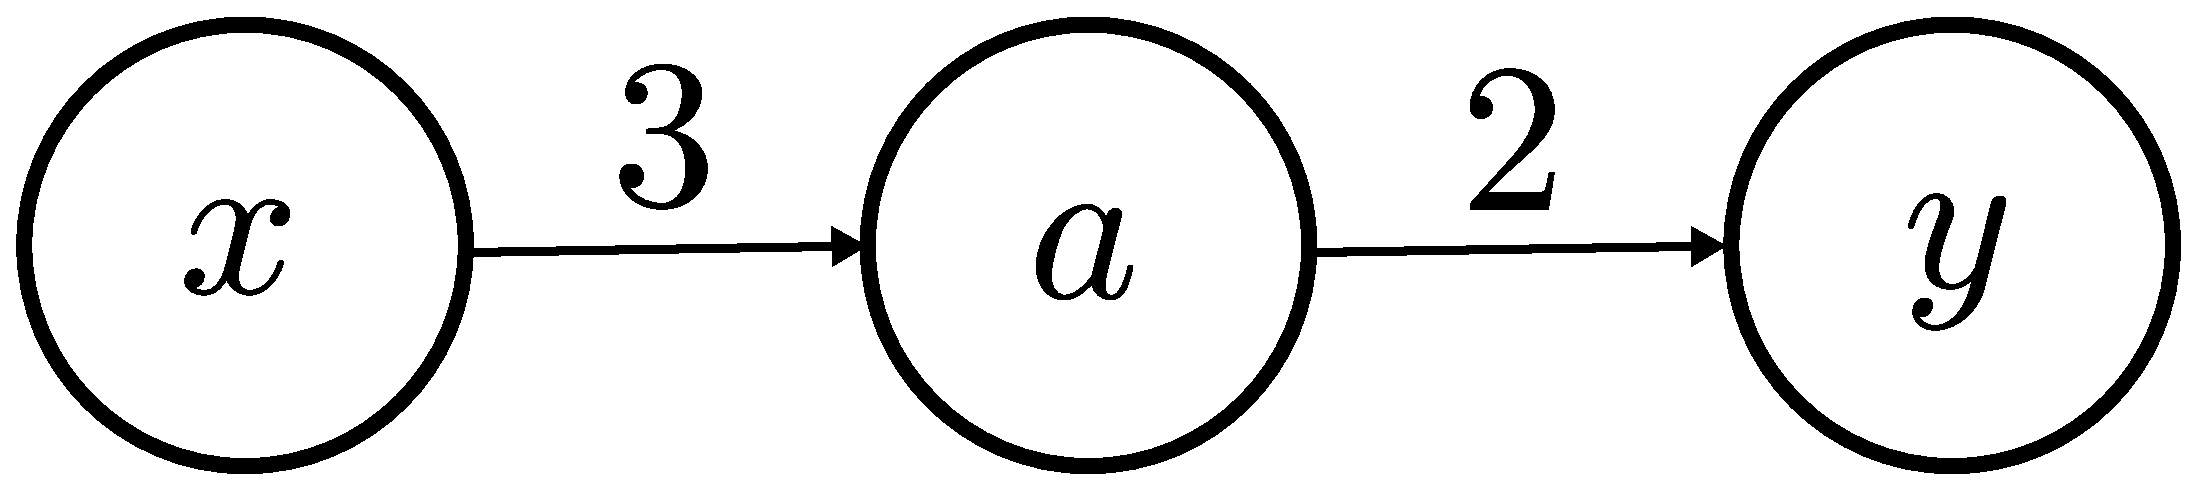
\includegraphics[width=0.3\textwidth]{./neural_networks_gradients_ex1.eps}
\caption{Example neural network}
\label{fig:ex1}
\end{figure}

Consider the simple case in Figure \ref{fig:ex1}. Here we use a graphical representation where each node (or vertex) is a value and the paths between nodes (or edges) is represented by a constant multiplied by the value from the previous node. So we can write these equations as:
\begin{align}
    y &= 2a \\
    a &= 3x
\end{align}

Of course, we could compose these functions and simply write $y=6x$, but we'll show the chain rule in this simplest case and quickly add complexity. We can write out the local derivatives for nodes $a$ and $y$.

\begin{align}
    \dfrac{\partial y}{\partial a} &= 2 \\
    \dfrac{\partial a}{\partial x} &= 3
\end{align}

Using the chain rule we have that

\begin{equation}
    \dfrac{\partial y}{\partial x} = \dfrac{\partial y}{\partial a} \dfrac{\partial a}{\partial x} = (2)(3) = 6
\end{equation}

As we move backward along a path, we apply the chain rule to "propagate" the derivative (the gradient) backwards through the graph. This is a key takeaway: along a path, we apply the chain rule.

\begin{figure}[h]
\centering
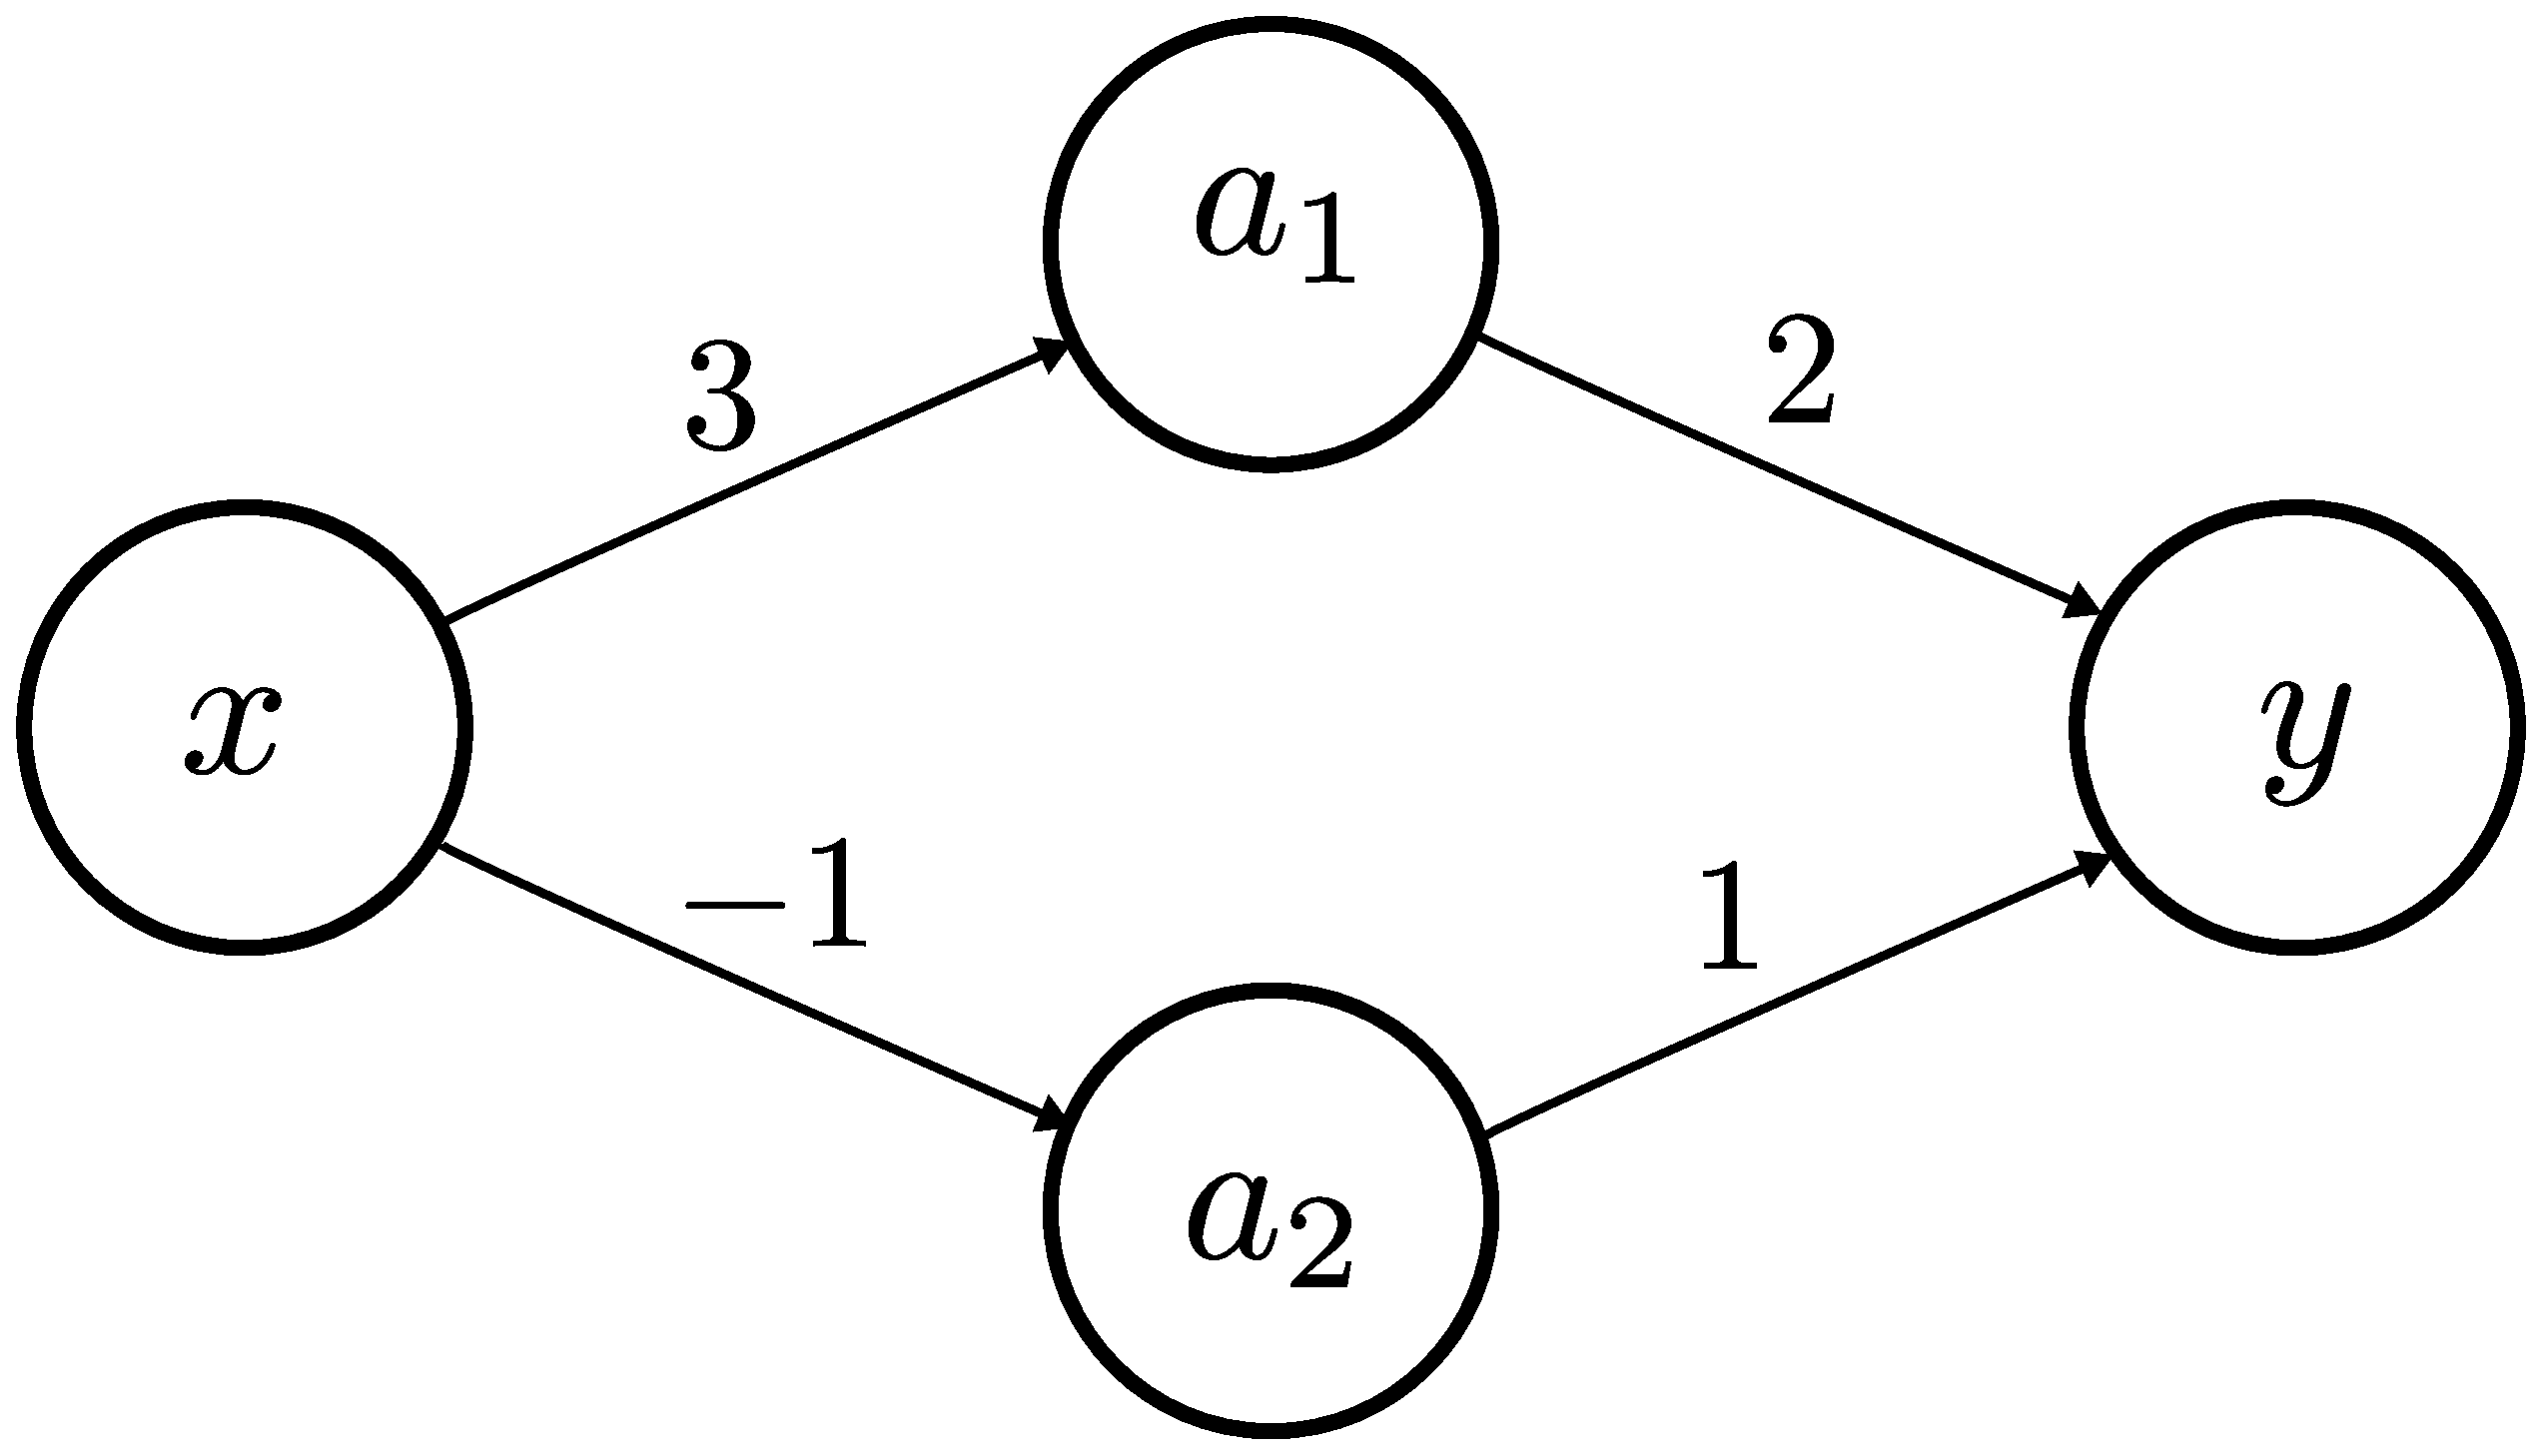
\includegraphics[width=0.3\textwidth]{./neural_networks_gradients_ex2.eps}
\caption{Example neural network}
\label{fig:ex2}
\end{figure}

In neural networks, we don't typically have this straight line from left to right, instead, there are multiple parallel pathways. Consider the example in Figure \ref{fig:ex2}. Here we can write out our three local equations for nodes $y$, $a_1$, and $a_2$:

\begin{align}
    y &= 2a_1 + a_2 \\
    a_1 &= 3x \\
    a_2 &= -x
\end{align}

If we tried to apply the chain rule directly, the fact that there are multiple paths connecting $x$ to $y$ becomes a challenge. But here we can use another important rule in calculus, the sum rule for differentiation:

\begin{equation}
    \dfrac{\partial}{\partial x} (a_1 + a_2) = \dfrac{\partial a_1}{\partial x} + \dfrac{\partial a_2}{\partial x}
\end{equation}

We can then apply the chain rule to $\frac{\partial a_1}{\partial x}$ and $\frac{\partial a_2}{\partial x}$ to get the derivative with respect to $x$:

\begin{equation}
\begin{split}
    \frac{\partial y}{\partial x} &= \frac{\partial y}{\partial a_1} \frac{\partial a_1}{\partial x} + \frac{\partial y}{\partial a_2} \frac{\partial a_2}{\partial x} \\
    &= (2)(3) + (1)(-1) \\
    &= 5
\end{split}
\end{equation}

To make sure this makes sense, we see that if we substitute in the values for $a_1$ and $a_2$ we get that $y=2(3x) - x = 5x$. Here we can clearly see that the derivative of $y$ with respect to $x$ is 5.

A key takeaway here is that when we encounter multiple parallel paths from one node to another, as in \ref{fig:ex2}, we have to add the contribution of the derivative from each of the paths that come out of one node. This combination of the sum rule and the chain rule for differentiation allow us to calculate the gradients in many different graphs where nodes feed forward into one another sequentially, such as with feedforward neural networks.

\begin{figure}[h]
\centering
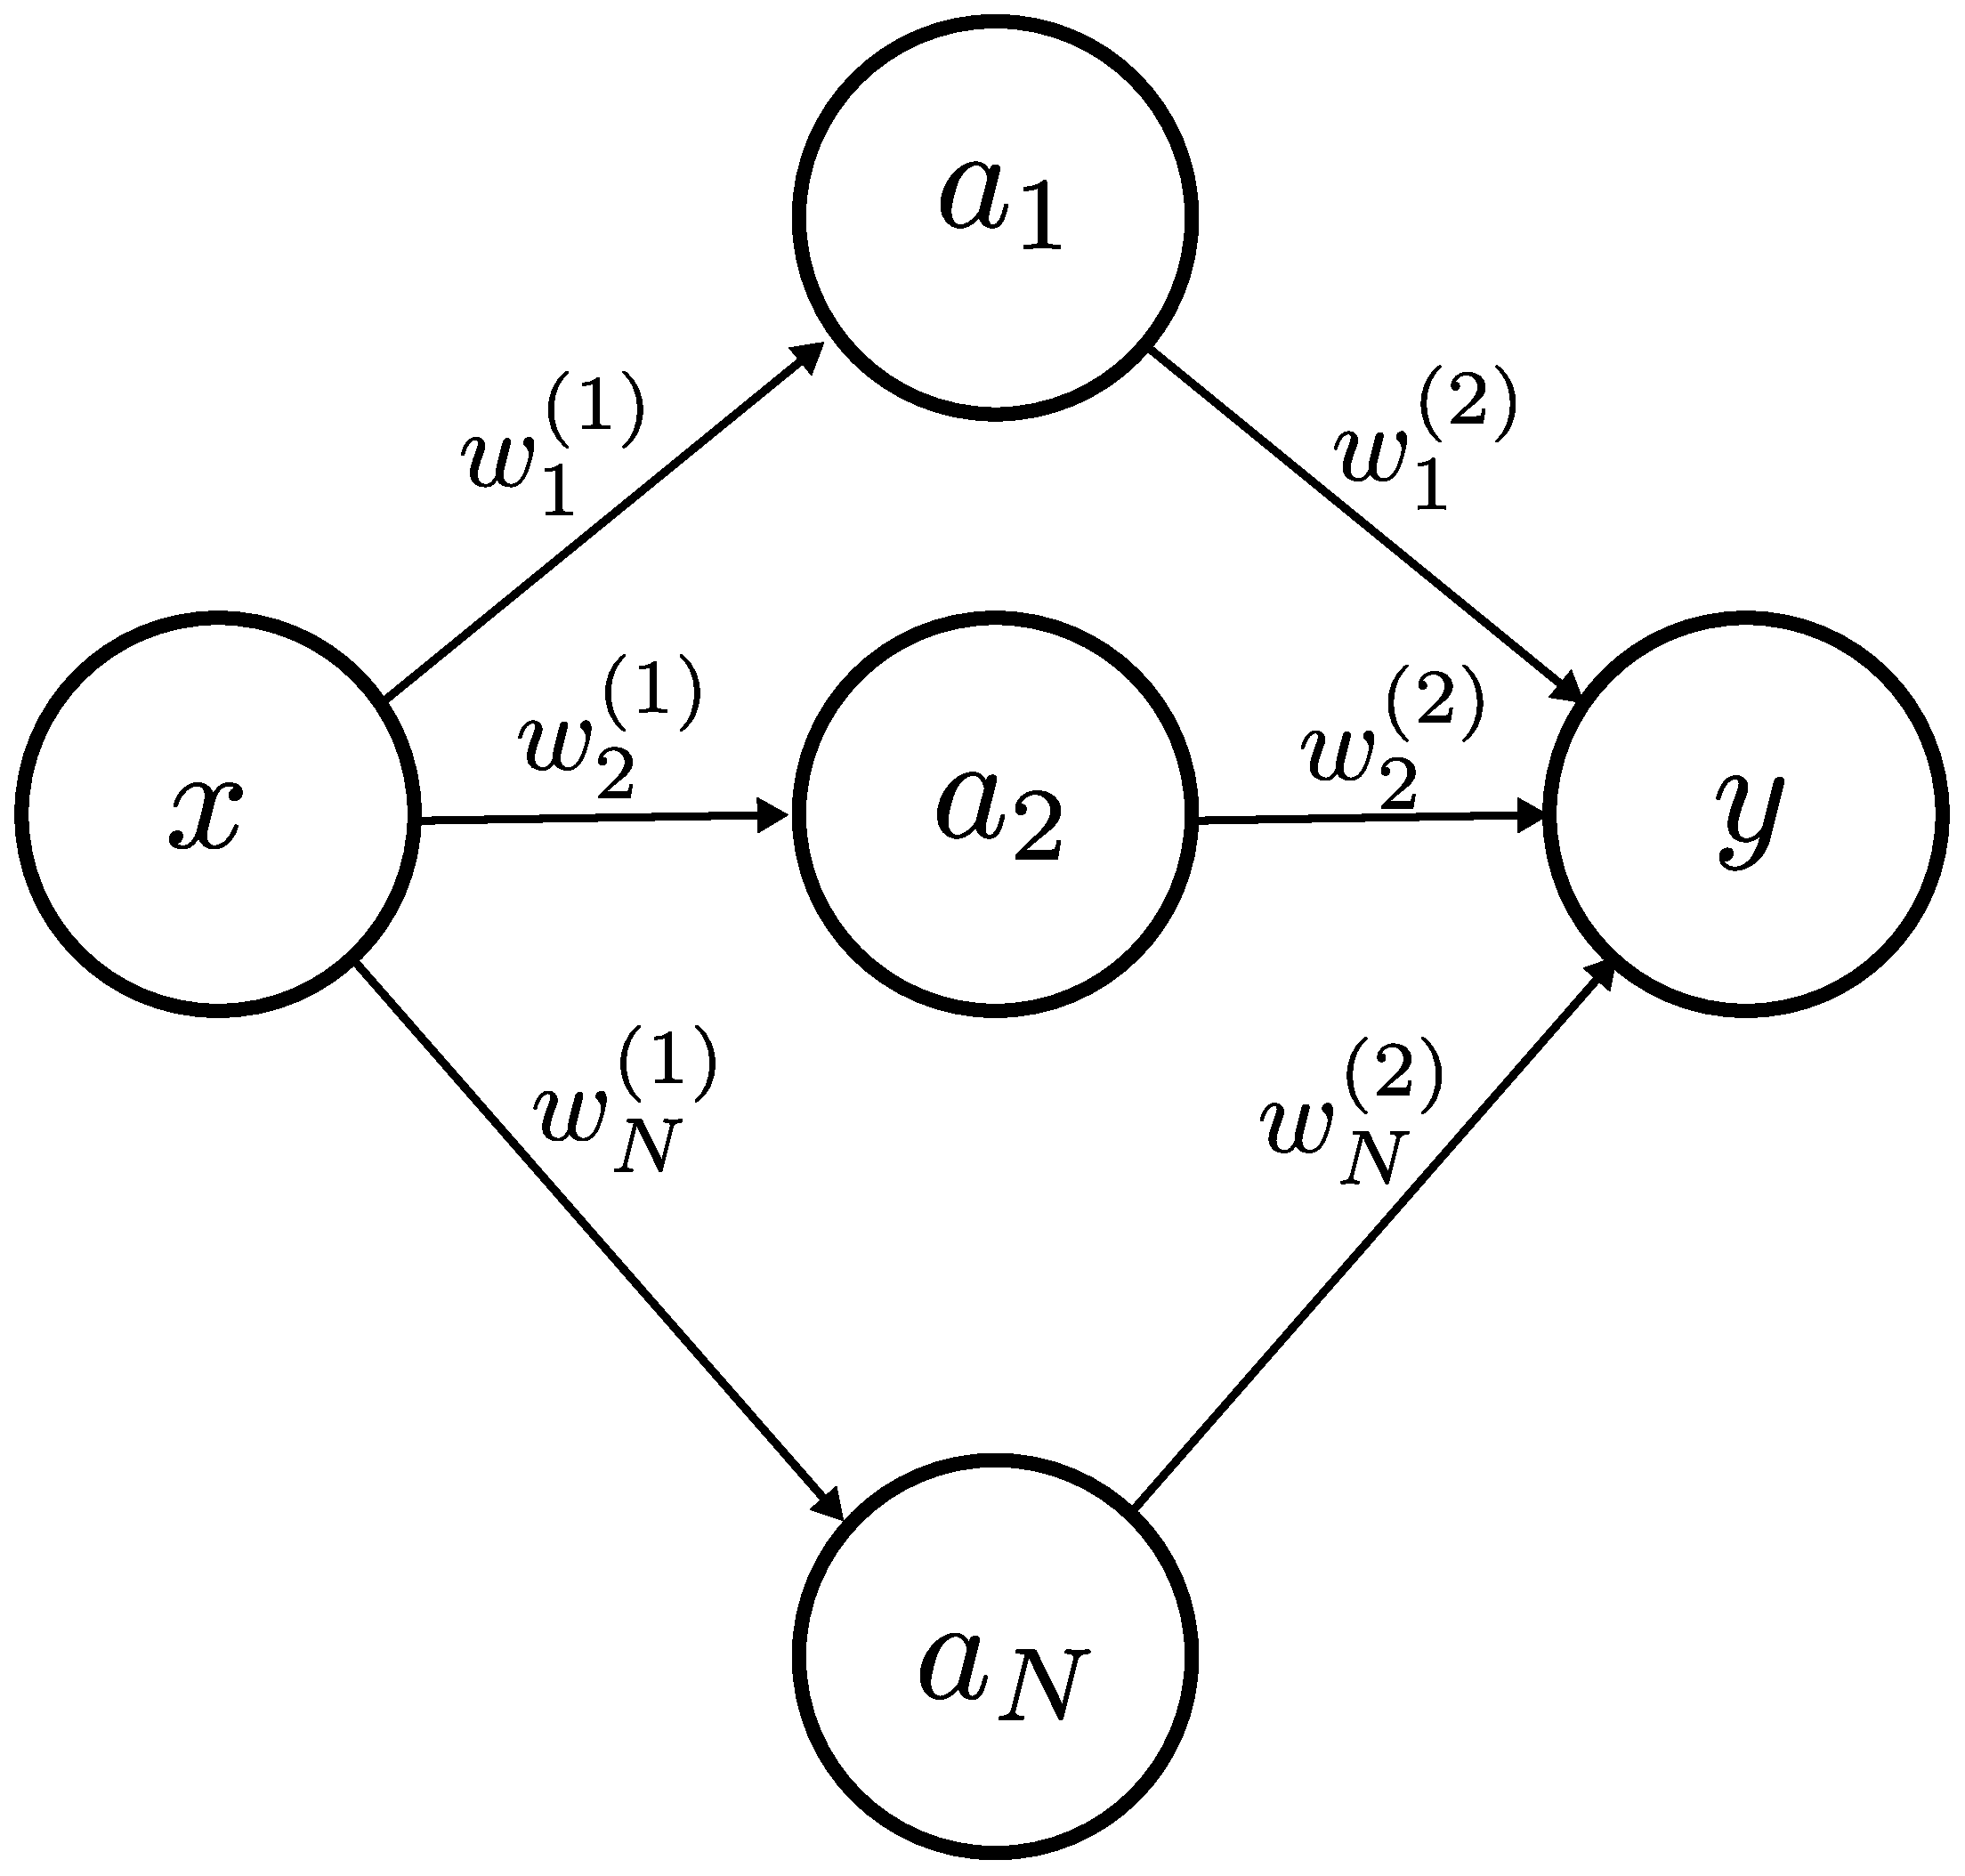
\includegraphics[width=0.3\textwidth]{./neural_networks_gradients_ex3.eps}
\caption{Example neural network}
\label{fig:ex3}
\end{figure}

Let's go through one slightly more complex example to get us ready for applying this directly to neural networks. Consider the situation in \ref{fig:ex3} that has $N$ paths from $x$ to $y$ instead of the earlier situations with only one or two described previously. Here the same combination of the sum rule across paths and the chain rule along paths can be applied. Let's start by righting our the relationships represented at each node once again.

Here we represent different layers in this network using the parenthetical superscript notation ($v^{(i)}$ being the value of $v$ for the $i$th layer).

\begin{align}
    y &= \sum\limits_j^N w_j^{(2)} a_j \\
    a_i &= w_i^{(1)} x
\end{align}

Now we can also write each of our local derivatives at each node:

\begin{align}
    \dfrac{\partial y}{\partial a_i} &= w_i^{(2)} \\
    \dfrac{\partial a_i}{\partial x} &= w_i^{(1)} \\
\end{align}

Then we can use the sum and chain rules to calculate the derivative of $y$ with respect to $x$:

\begin{align}
    \dfrac{\partial y}{\partial x} &= \sum\limits_{j=1}^N  \dfrac{\partial y}{\partial a_j} \dfrac{\partial a_j}{\partial x} \label{eq:ex3_der}\\
    &= \sum\limits_{j=1}^N w_j^{(2)} w_j^{(1)}
\end{align}

Now if we wanted to get the derivative of $y$ with respect to any of the weights, that's easy since we have all the pieces ready. For $w_i^{(2)}$ this is:

\begin{equation}
    \dfrac{\partial y}{\partial w_i^{(2)}} = \dfrac{\partial}{\partial w_i^{(2)}}  \left(\sum\limits_j^N w_j^{(2)} a_j \right) = a_i
    \label{eq:dw2}
\end{equation}

This simplifies since the derivatives are all zero except for when $j=i$ in \ref{eq:dw2}.To calculate $w_i^{(2)}$, we just need one more application of the chain rule:

\begin{align}
    \dfrac{\partial y}{\partial w_i^{(1)}} &= \dfrac{\partial y}{\partial a_i} \dfrac{\partial a_i}{\partial w_i^{(1)}} \\
    &= (w_i^{(2)})(x)
\end{align}

This is because we defined $\frac{\partial y}{\partial a_i}$ above in \ref{eq:ex3_der} and since $a_i = w_i^{(1)} x$, then $\frac{\partial a_i}{\partial w_i^{(1)}} = x$.

This concept of using the chain rule along paths and the sum rule across paths is all that's needed for backpropagation in neural networks. And all backpropagation does is allows us to calculate the derivative of our loss function with respect to every parameter in the neural network. We can then use those values to adjust our weight parameters and improve the fit of our model.

\section{The math behind backpropagation through a simple example}

Let's apply these techniques to a simple example of a neural network and calculate the gradients of its error with respect to every parameter. While neural networks are highly customizable in terms of the number of hidden layers and the number of nodes in each layer, we'll use an example of a neural network with two hidden layers with two nodes in each layer as shown in Figure \ref{fig:nnexample}.

\begin{figure}[h]
\centering
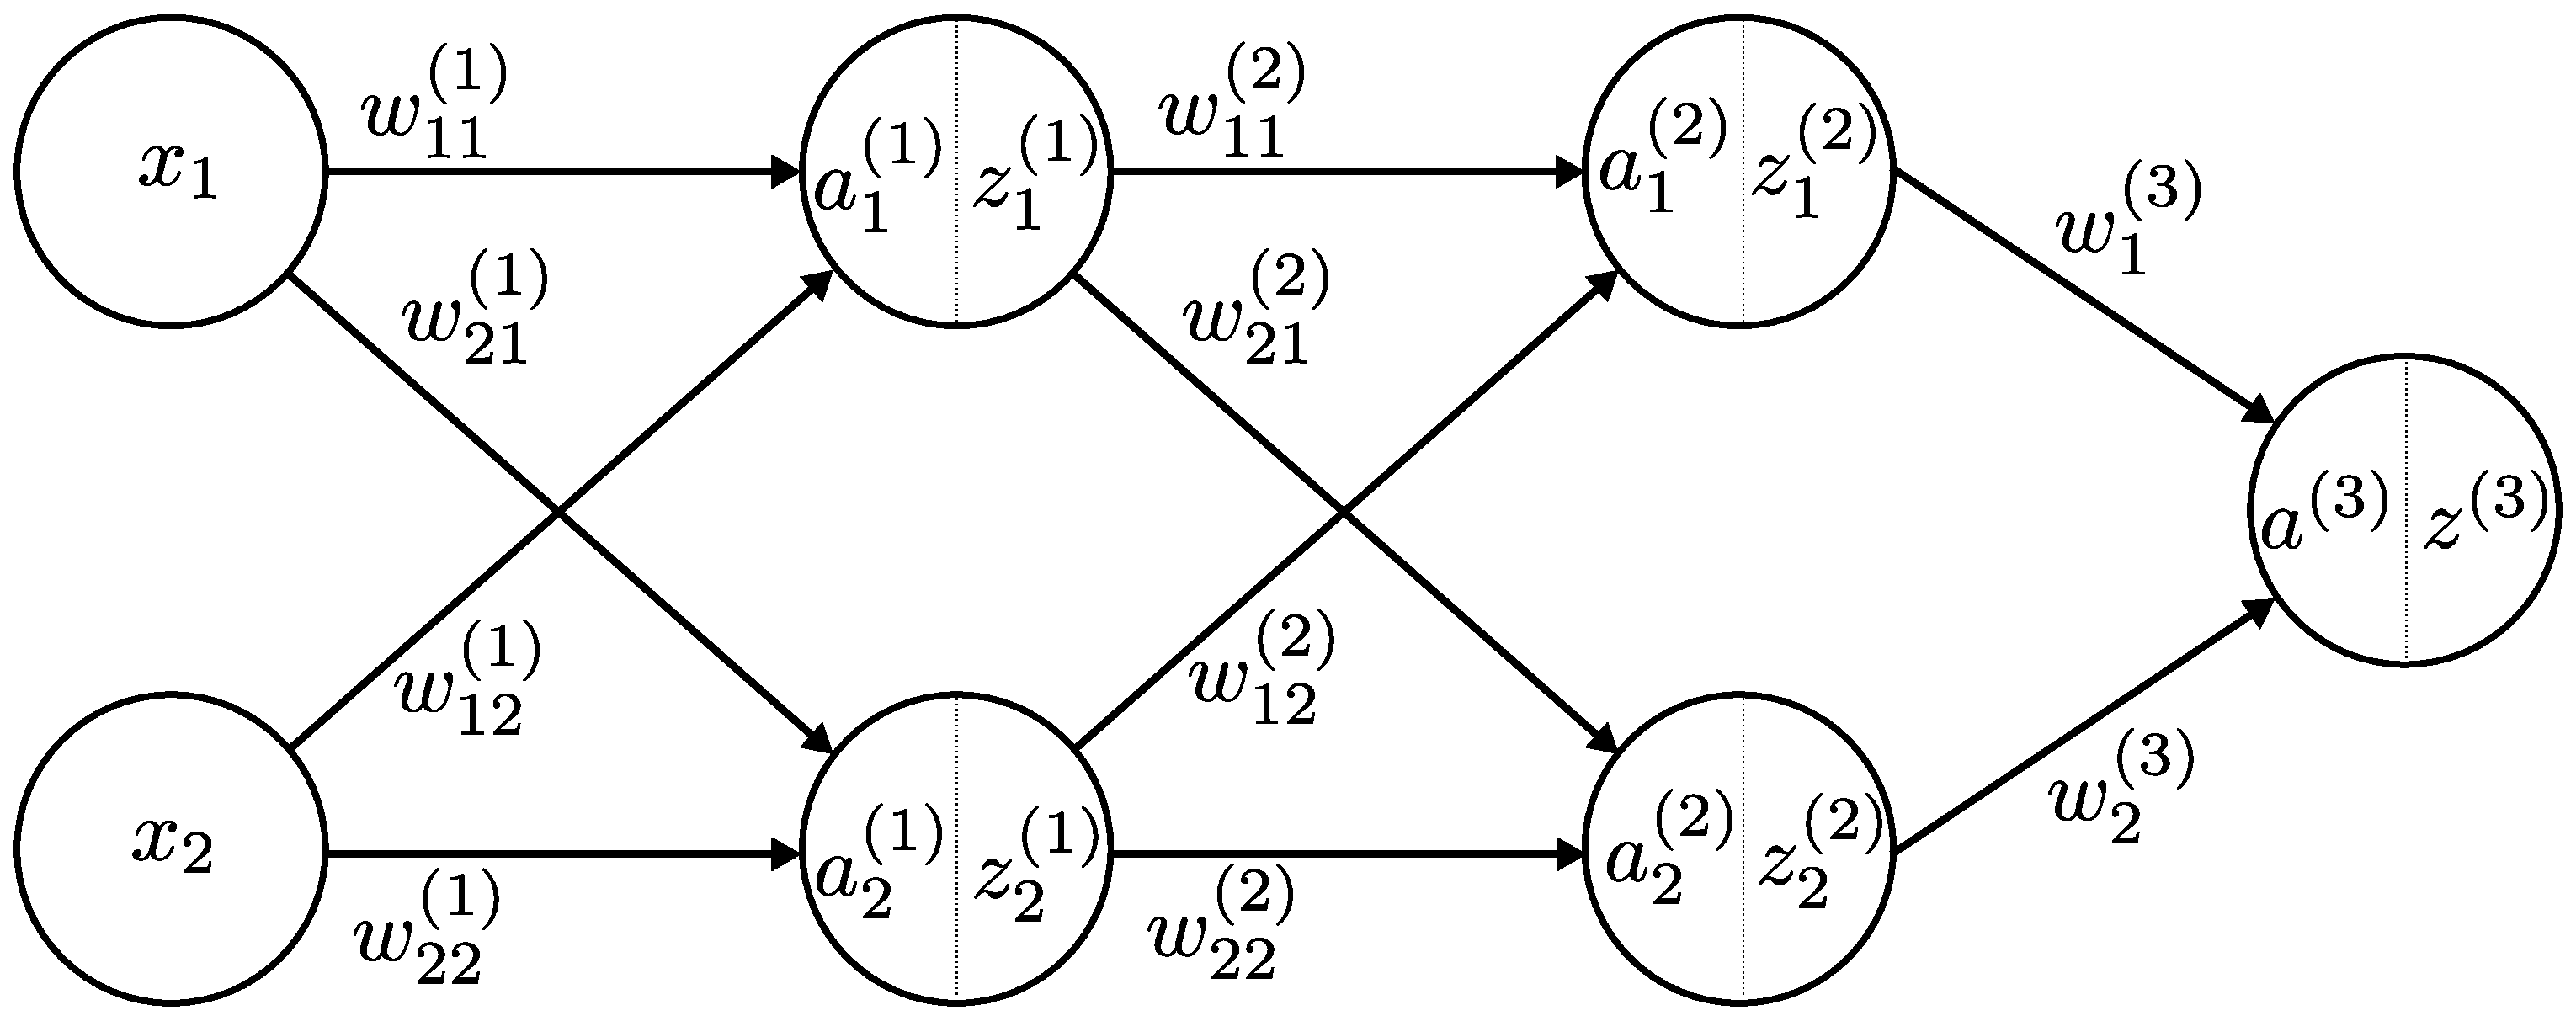
\includegraphics[width=0.9\textwidth]{./neural_networks.eps}
\caption{Example neural network. A 3-layer network with two hidden layers and one output node. The final layer doesn't have subscripts for simplicity and the final set of weights also only have one subscript each to keep the notation simple, but are otherwise the same as all other nodes in the neural network.}
\label{fig:nnexample}
\end{figure}

\subsection{Feeding inputs forward through the network}

Let's start by defining what all of the pieces here mean. We have our inputs $x_i$, which we'll also refer to as the zero-th layer, so $z_i^{(0)} \triangleq x_i $. between the layers we have each set of weights, so $w_{ij}^{(k)}$ represents the weight from node $j$ in layer $k-1$ to node $i$ in layer $k$. Each hidden layer is comprised of two parts (which are separated by a dotted line in Figure \ref{fig:nnexample}), the activations $a_i^{(k)}$ and the hidden node values $z_i^{(k)}$. The activations are the sum of the incoming paths into the node: the value of the last layer times the weight along the path. For example, $a_1^{(1)}=x_1 w_{11}^{(1)} + x_2 w_{12}^{(2)}$. The hidden node values are then the activations transformed by an activation function. While there are many choices for this including sigmoids, hyperbolic tangent, and more recently rectified linear units (ReLU), we'll represent the general case of activations with $\sigma(\cdot)$. In this tutorial, we'll assume that $\sigma(\cdot)$ is a sigmoid function ($\sigma(x) = \frac{1}{1+e^{-x}}$. Using this, the hidden node value can be defined as:

\begin{equation}
    z_i^{(k)} = \sigma(a_i^{(k)})
\end{equation}

So for our example in in Figure \ref{fig:nnexample} with $a_1^{(1)}$, we could write out the expression to "feed forward" from one layer into the next in one line:

\begin{equation}
    z_1^{(k)} = \sigma(a_i^{(k)}) = \sigma(x_1 w_{11}^{(1)} + x_2 w_{12}^{(2)})
\end{equation}

\begin{figure}[h]
\centering
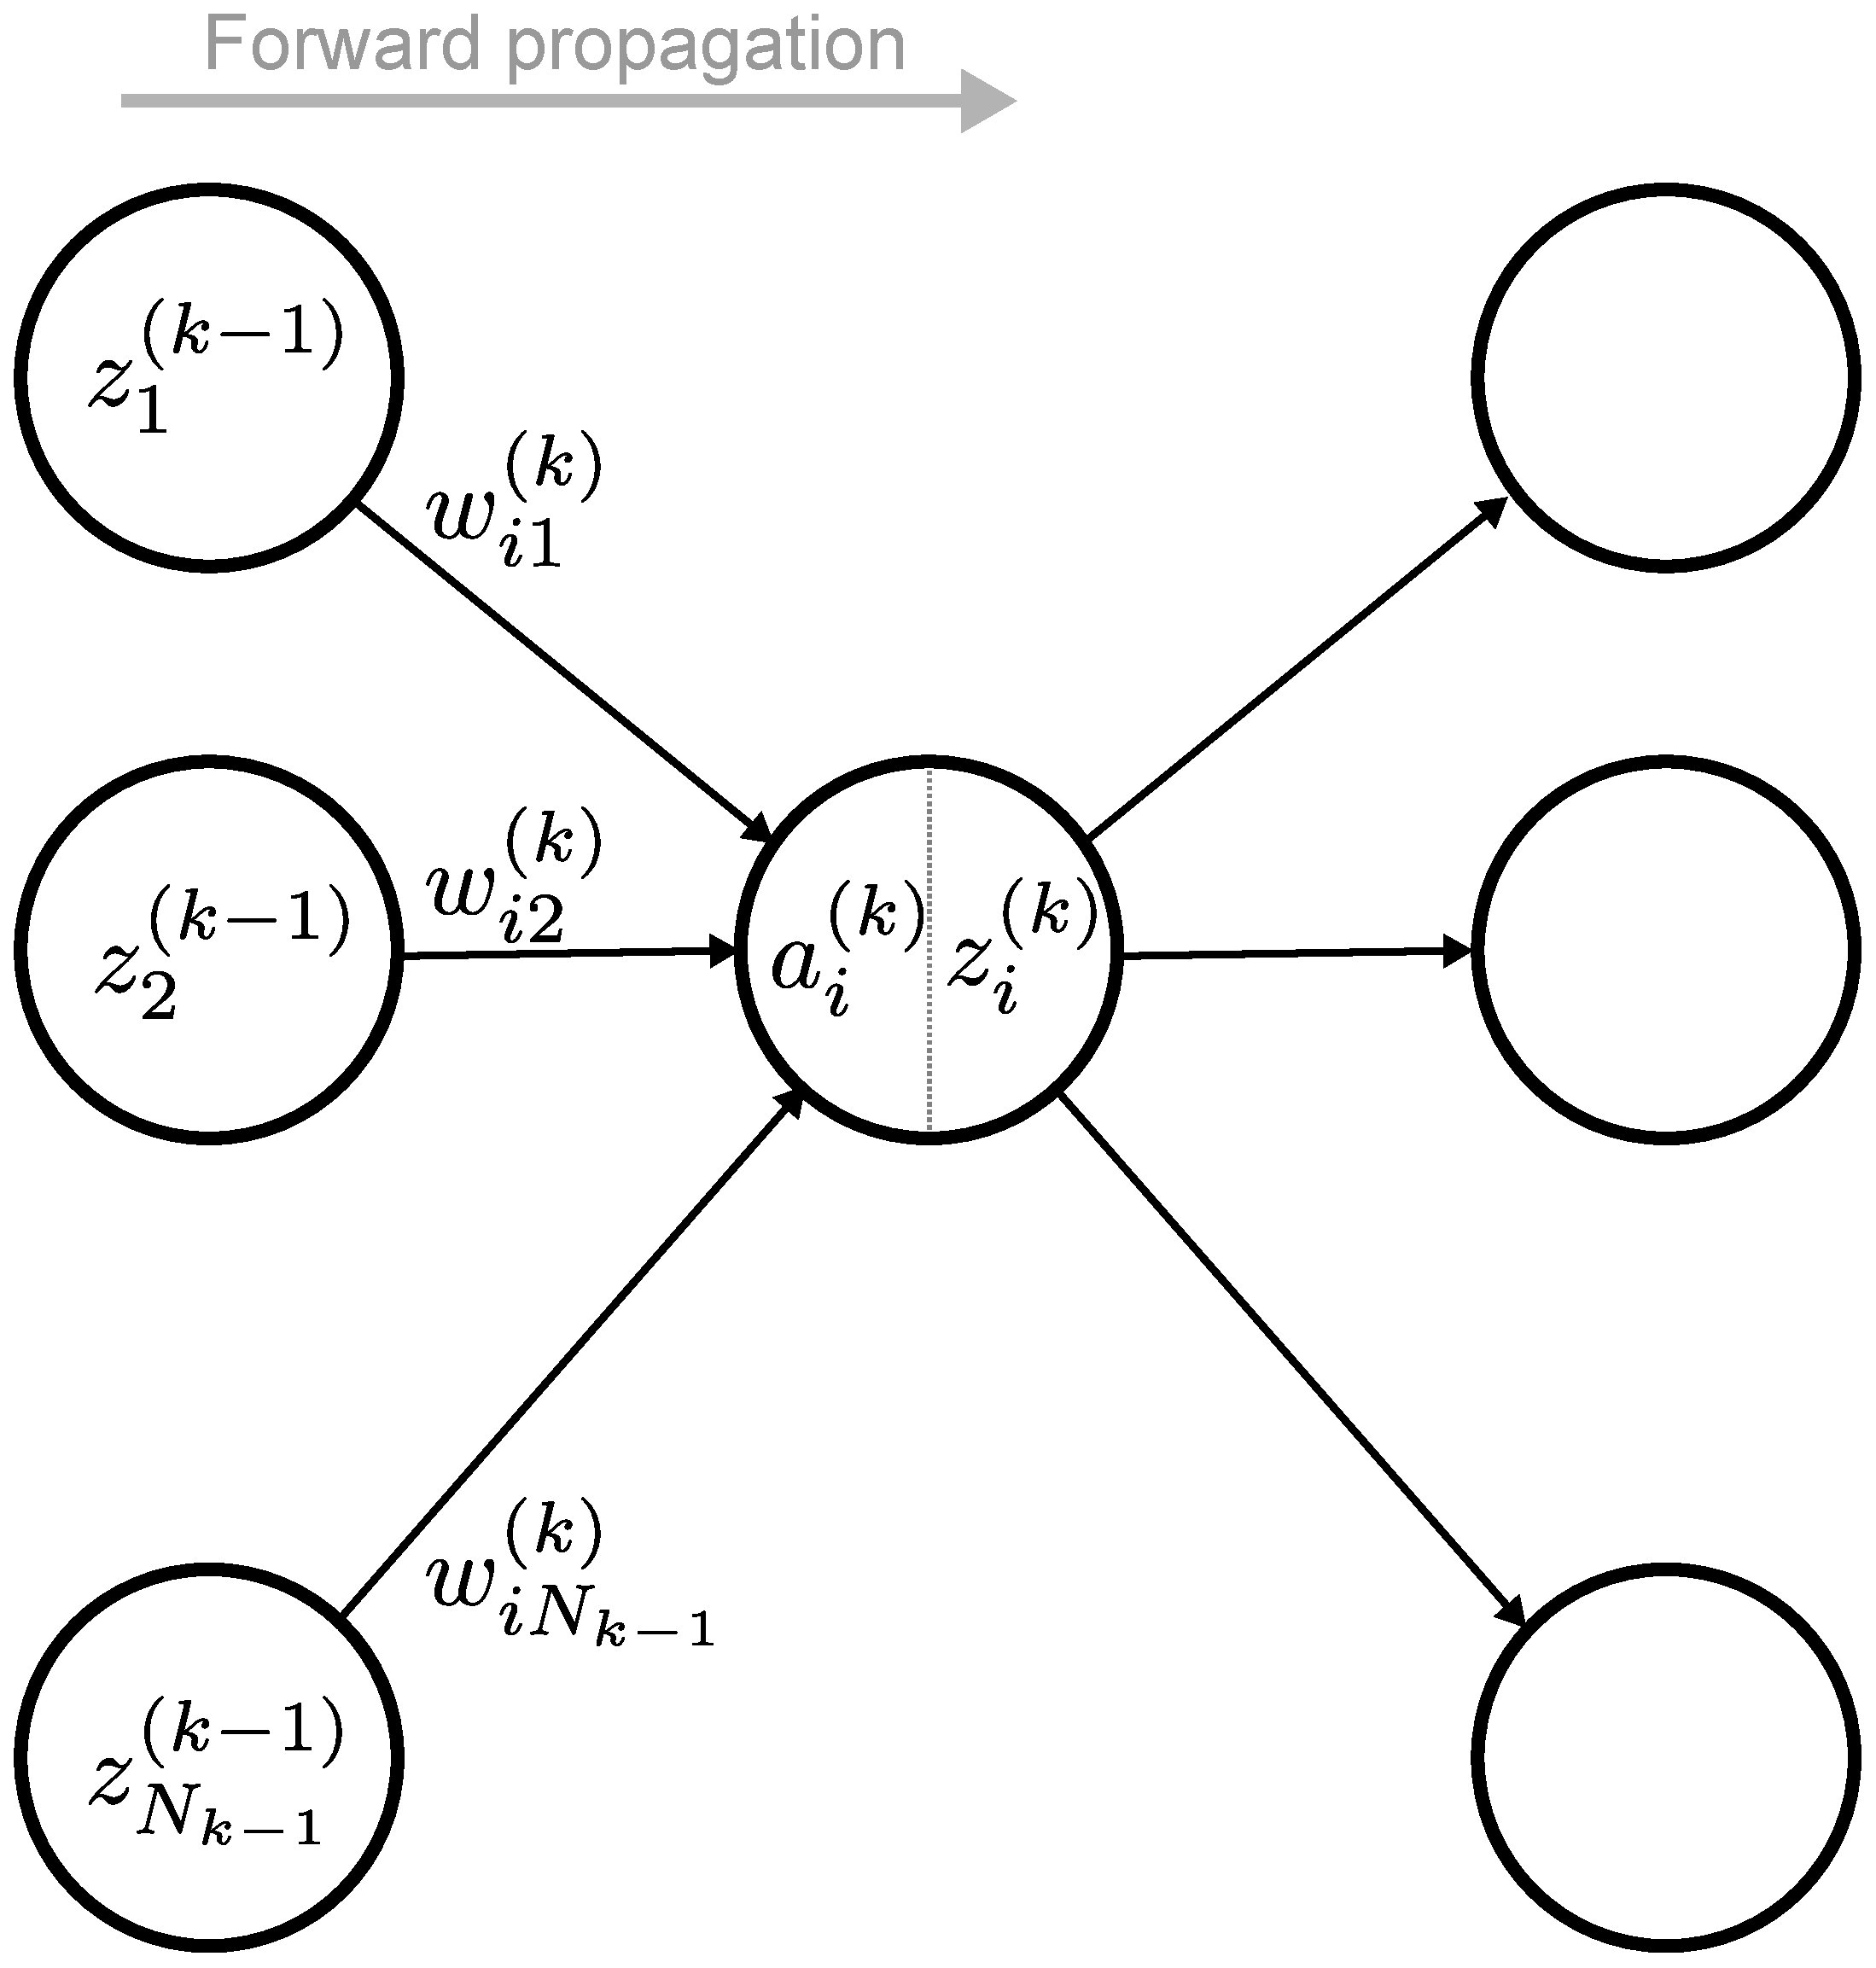
\includegraphics[width=0.45\textwidth]{./neural_networks_local_forward_propagation.eps}
\caption{Example neural network}
\label{fig:ff}
\end{figure}

We can do this for all of the nodes in the neural network feeding each layer forward into the next as demonstrated in Figure \ref{fig:ff}. More generally, we can write:

\begin{equation}
    a_i^{(k)} = \sum_{j=1}^{N_{k-1}} w_{ij}^{(k)} z_j^{(k-1)} 
\end{equation}

and

\begin{equation}
    z_i^{(k)} = \sigma(a_i^{(k)})
\end{equation}

Which collectively feed each layer forward to the next. This will fully populate the neural network values for a given set of weights. Let's adopt a matrix notation to store these and right them all out:

\begin{equation}
\mathbf{x} = 
    \begin{bmatrix}
        x_{1}\\
        x_{2}\\
        \vdots\\
        x_{N_{0}}\\
    \end{bmatrix}, \quad
    \mathbf{a}^{(k)} = 
    \begin{bmatrix}
        a_1^{(k)}\\
        a_2^{(k)}\\
        \vdots\\
        a_{N_k}^{(k)}\\
    \end{bmatrix}, \quad
    \mathbf{z}^{(k)} = 
    \begin{bmatrix}
        z_1^{(k)}\\
        z_2^{(k)}\\
        \vdots\\
        z_{N_k}^{(k)}\\
    \end{bmatrix}, \quad
    \mathbf{W}^{(k)} = 
    \begin{bmatrix}
        w_{11}^{(k)} & w_{12}^{(k)} & \cdots & w_{1 N_k}^{(k)}\\[2ex]
        w_{21}^{(k)} & w_{22}^{(k)} & \cdots & w_{2 N_k}^{(k)}\\[2ex]
        \vdots & \vdots &  & \vdots\\[2ex]
        w_{N_{k+1} 1}^{(k)} & w_{N_{k+1} 2}^{(k)} & \cdots & w_{N_{k+1} N_k }^{(k)}\\[2ex]
    \end{bmatrix}
\end{equation}

Each layer has its own collection of activations, hidden node values, and weights as shown in Figure \ref{fig:fullnn}, where we assume we have $K$ layers (we typically don't count the input layer in the layer count. There are $K-1$ hidden layers and a final output layer. In the regression setting, there may be a different activation function present in the final output layer, or even no activation function at all. In this example, we'll assume we're using mean square error as our error metric and a sigmoid activation for all hidden and output layers. The layers can be different sizes, each with $N_k$ nodes. Regardless of the number of nodes per layer and the number of layers, the math for calculating the output from an input and the gradients along the way remains the same and can be written in just a few equations.

\begin{figure}[h]
\centering
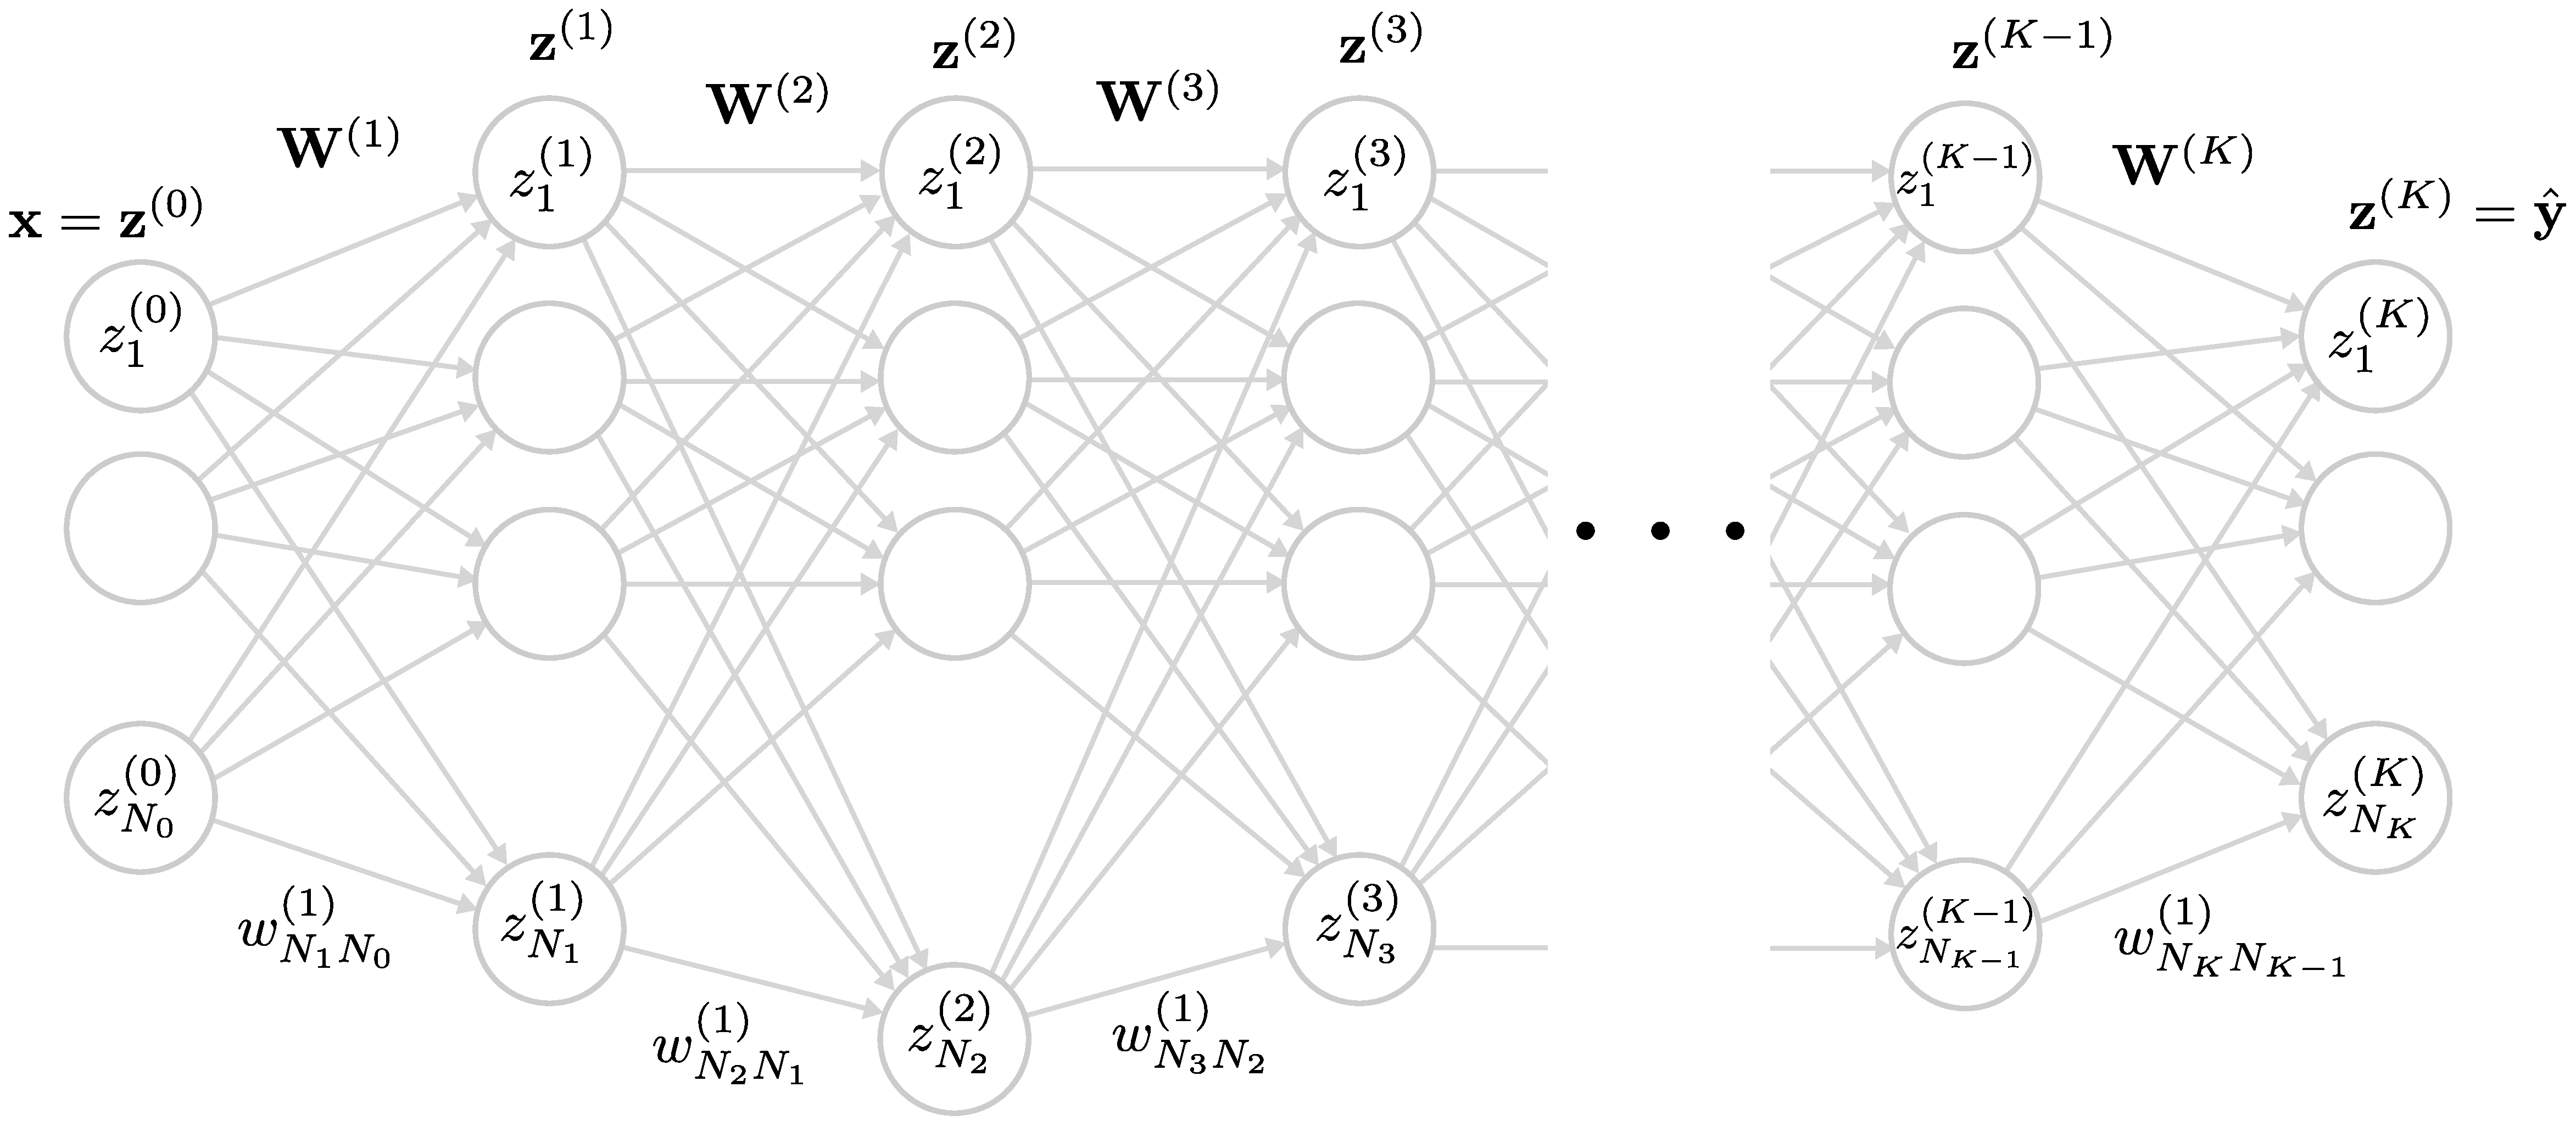
\includegraphics[width=0.9\textwidth]{./neural_networks_full_with_labels.eps}
\caption{Example neural network}
\label{fig:fullnn}
\end{figure}

Let's focus in on a particular node in the network and use that as representative. We'll focus on the $i$th node in the $k$th layer as shown in Figure \ref{fig:focused}. What we can see in this figure is that all of the nodes of the previous layer are inputs into this node, with a corresponding weight, and are therefore needed to calculate the value of $x_i^{k}$. Additionally, this node is an input (one of many) into every one of the values in the next layer of the network.

\begin{figure}[h]
\centering
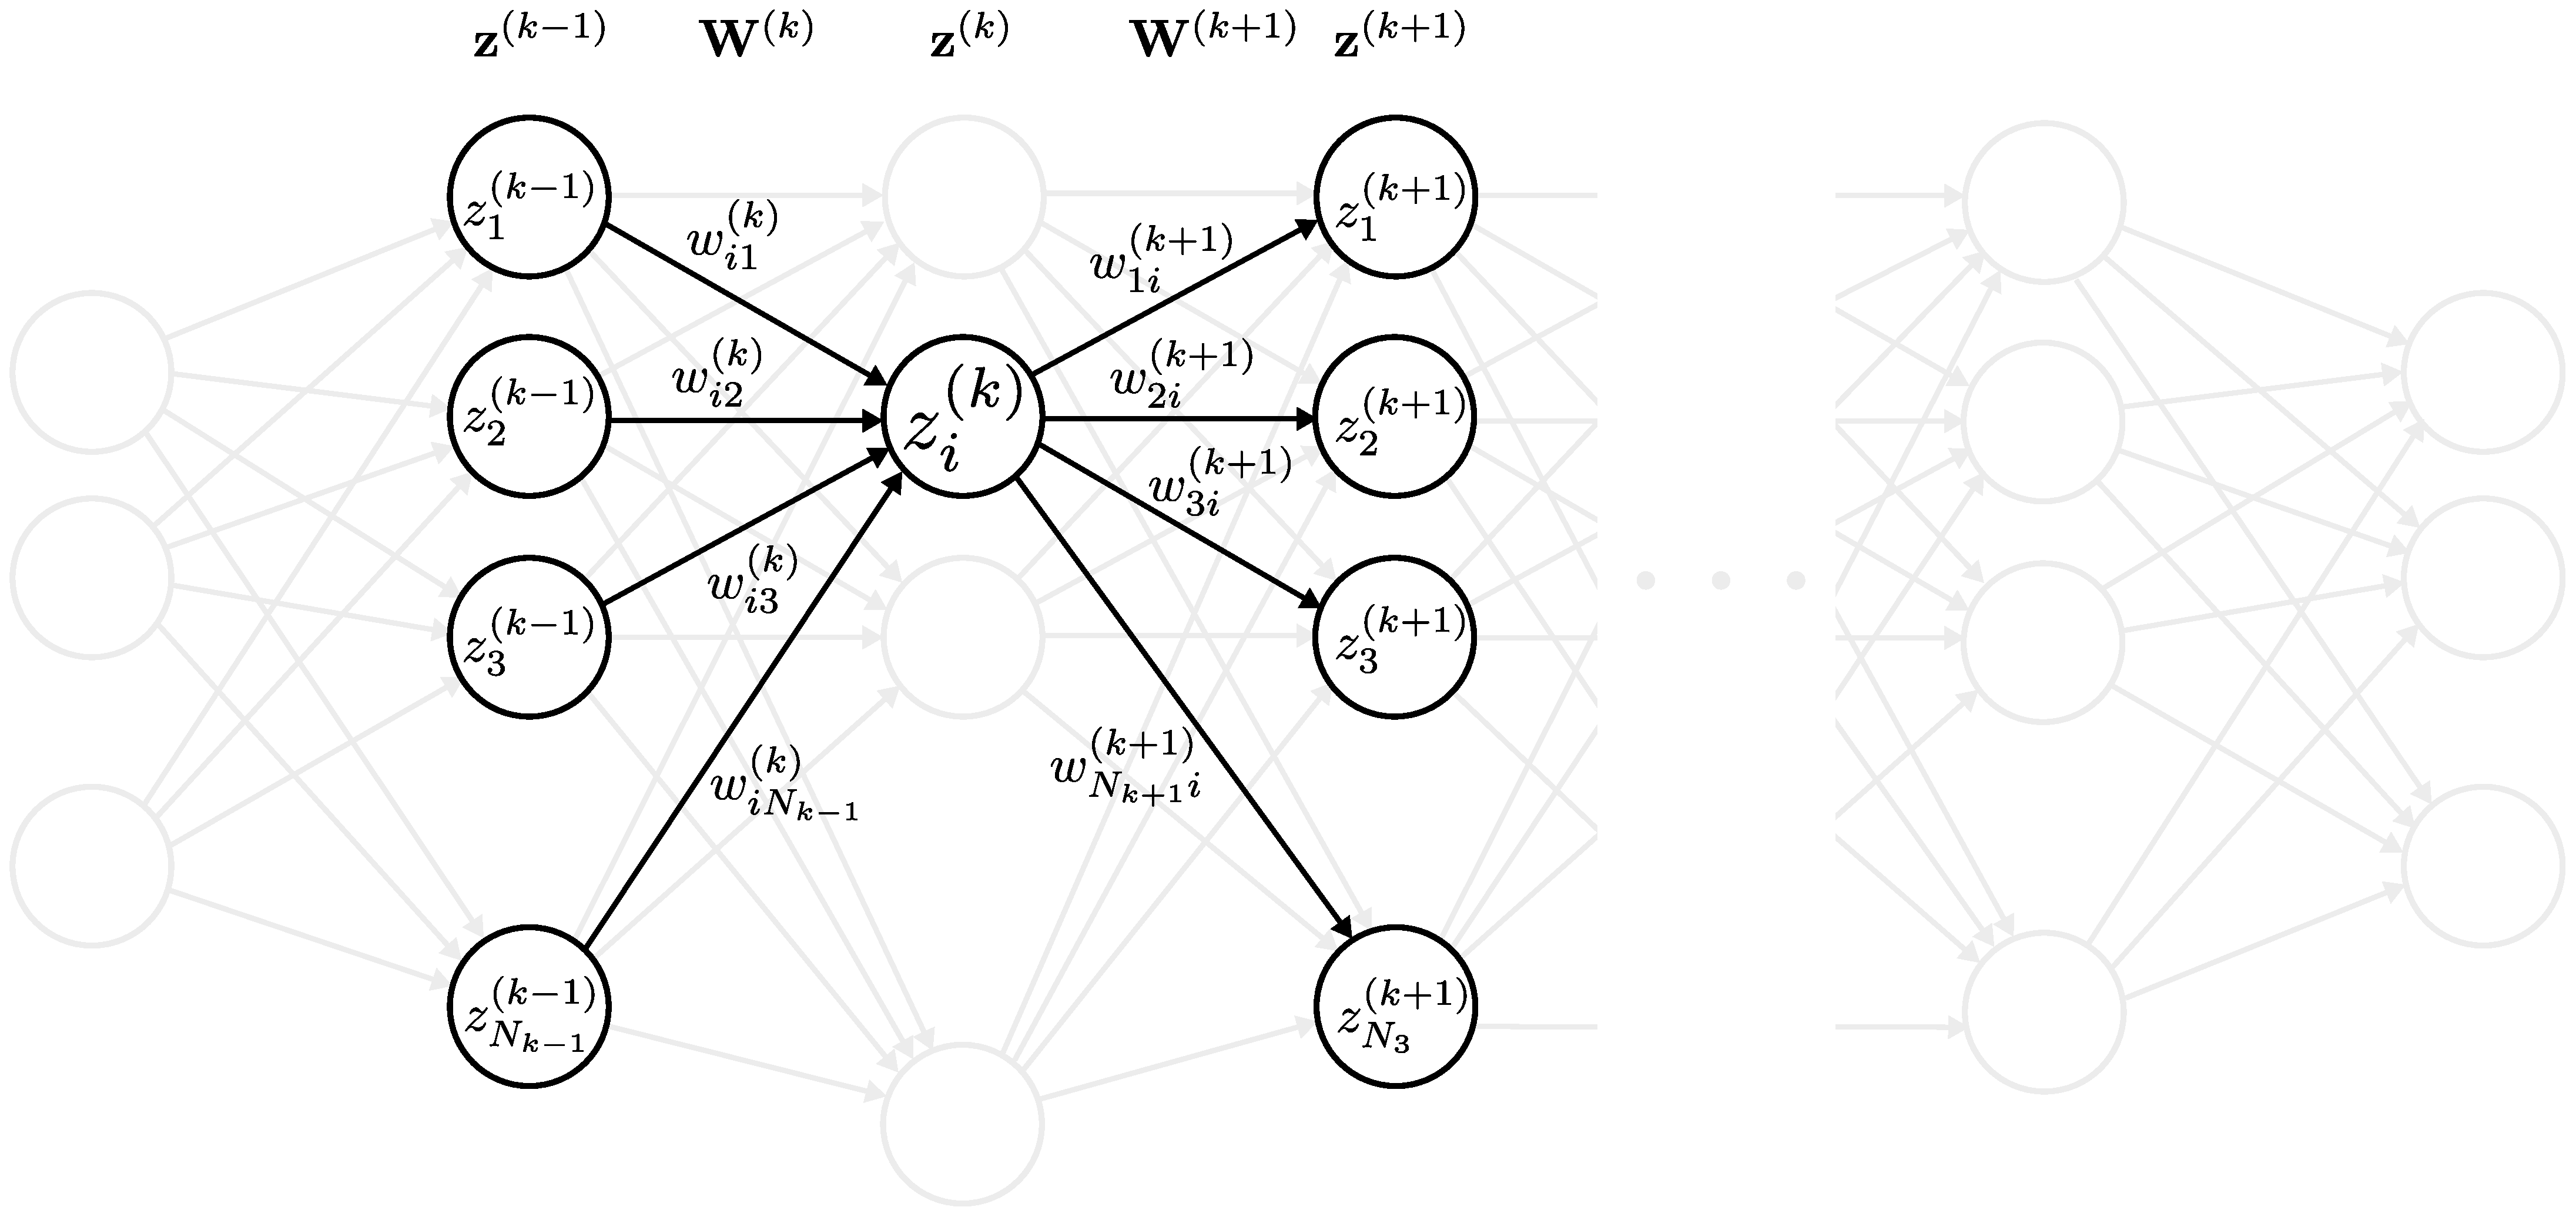
\includegraphics[width=0.9\textwidth]{./neural_networks_full_focused_example.eps}
\caption{Example neural network}
\label{fig:focused}
\end{figure}

This means that we can compute the value of each node in a proceeding layer as the linear combination of the node values of the last layer and the weights into the current node. This is shown in Figure \ref{fig:ff} and given by this relationships: 

\begin{equation}
    a_i^{(k)} = \sum_{j=1}^{N_{k-1}} w_{ij}^{(k)} z_j^{(k-1)} 
\end{equation}

Or in matrix form:

\begin{equation}
    \mathbf{a}^{(k)} = \mathbf{W}^{(k)} \mathbf{z}^{(k-1)}
\end{equation}

Then we can simply apply the activation function to this activation value:

\begin{equation}
    z_i^{(k)} = \sigma(a_i^{(k)})
\end{equation}

Or to all the activation values in matrix form. This function would be an element-wise operation of the activation function on each element of $\mathbf{a}^{(k)}$.

\begin{equation}
    \mathbf{z}^{(k)} = \sigma(\mathbf{a}^{(k)})
\end{equation}

Once we feed this all the way forward, we produce an output $\hat{\mathbf{y}} = \mathbf{z}^{(K)}$. We could use this as our prediction for the corresponding input $\mathbf{x}$.



\subsection{Backpropagation}

Once we have a prediction, if it's not a perfect prediction, there will be a difference between the prediction $\hat{\mathbf{y}}$ and out target value $\mathbf{y}$, resulting in an error. While there are a number of ways to measure error (often mean square error for regression and cross entropy for classification), we can compute the error resulting from the input training sample $\mathbf{x}_n$ and call it $E_n$. Our goal in the training process is to update the weights of the neural network function to minimize this error. To do so, we can use gradient descent were we move the value of each weight in the direction indicated by the gradient would most reduce error. Our gradient descent update equation is typically:

\begin{equation}
    w_i \leftarrow w_i - \lambda \dfrac{\partial E_n}{\partial w_i}
\end{equation}

Here, $\lambda$ is the learning rate, or how much to move the parameter $w_i$ for one step in the algorithm. Typically we'd apply a variant of stochastic gradient descent where we would randomly select a training data point from the training dataset (without replacement), feed it forward through the network, calculate the error compared to the target value, then compute the gradient with respect to every weight parameter in the network and use the above equation to adjust each parameter a little in the direction suggested by the gradient. Note that we move in the direction opposite to the gradient since the gradient points in the direction of steepest ascent and we want steepest descent.

How do we calculate the gradient of the error with respect to each weight in the network, though? When we discussed the application of the sum and chain rule to calculate the derivative of a function, we saw that we can compute all the gradients by applying the chain rule along paths, and the sum rule across parallel paths. We'll use that idea once again. Here we'll walk through calculating the gradient for every quantity in Figure \ref{fig:labeled_backprop}. Along the top of that figure each stage in the backpropagation process is numbered for reference. Every equation of the backpropagation process is written out in detail in Table \ref{tab:backprop}.

\begin{figure}[h]
\centering
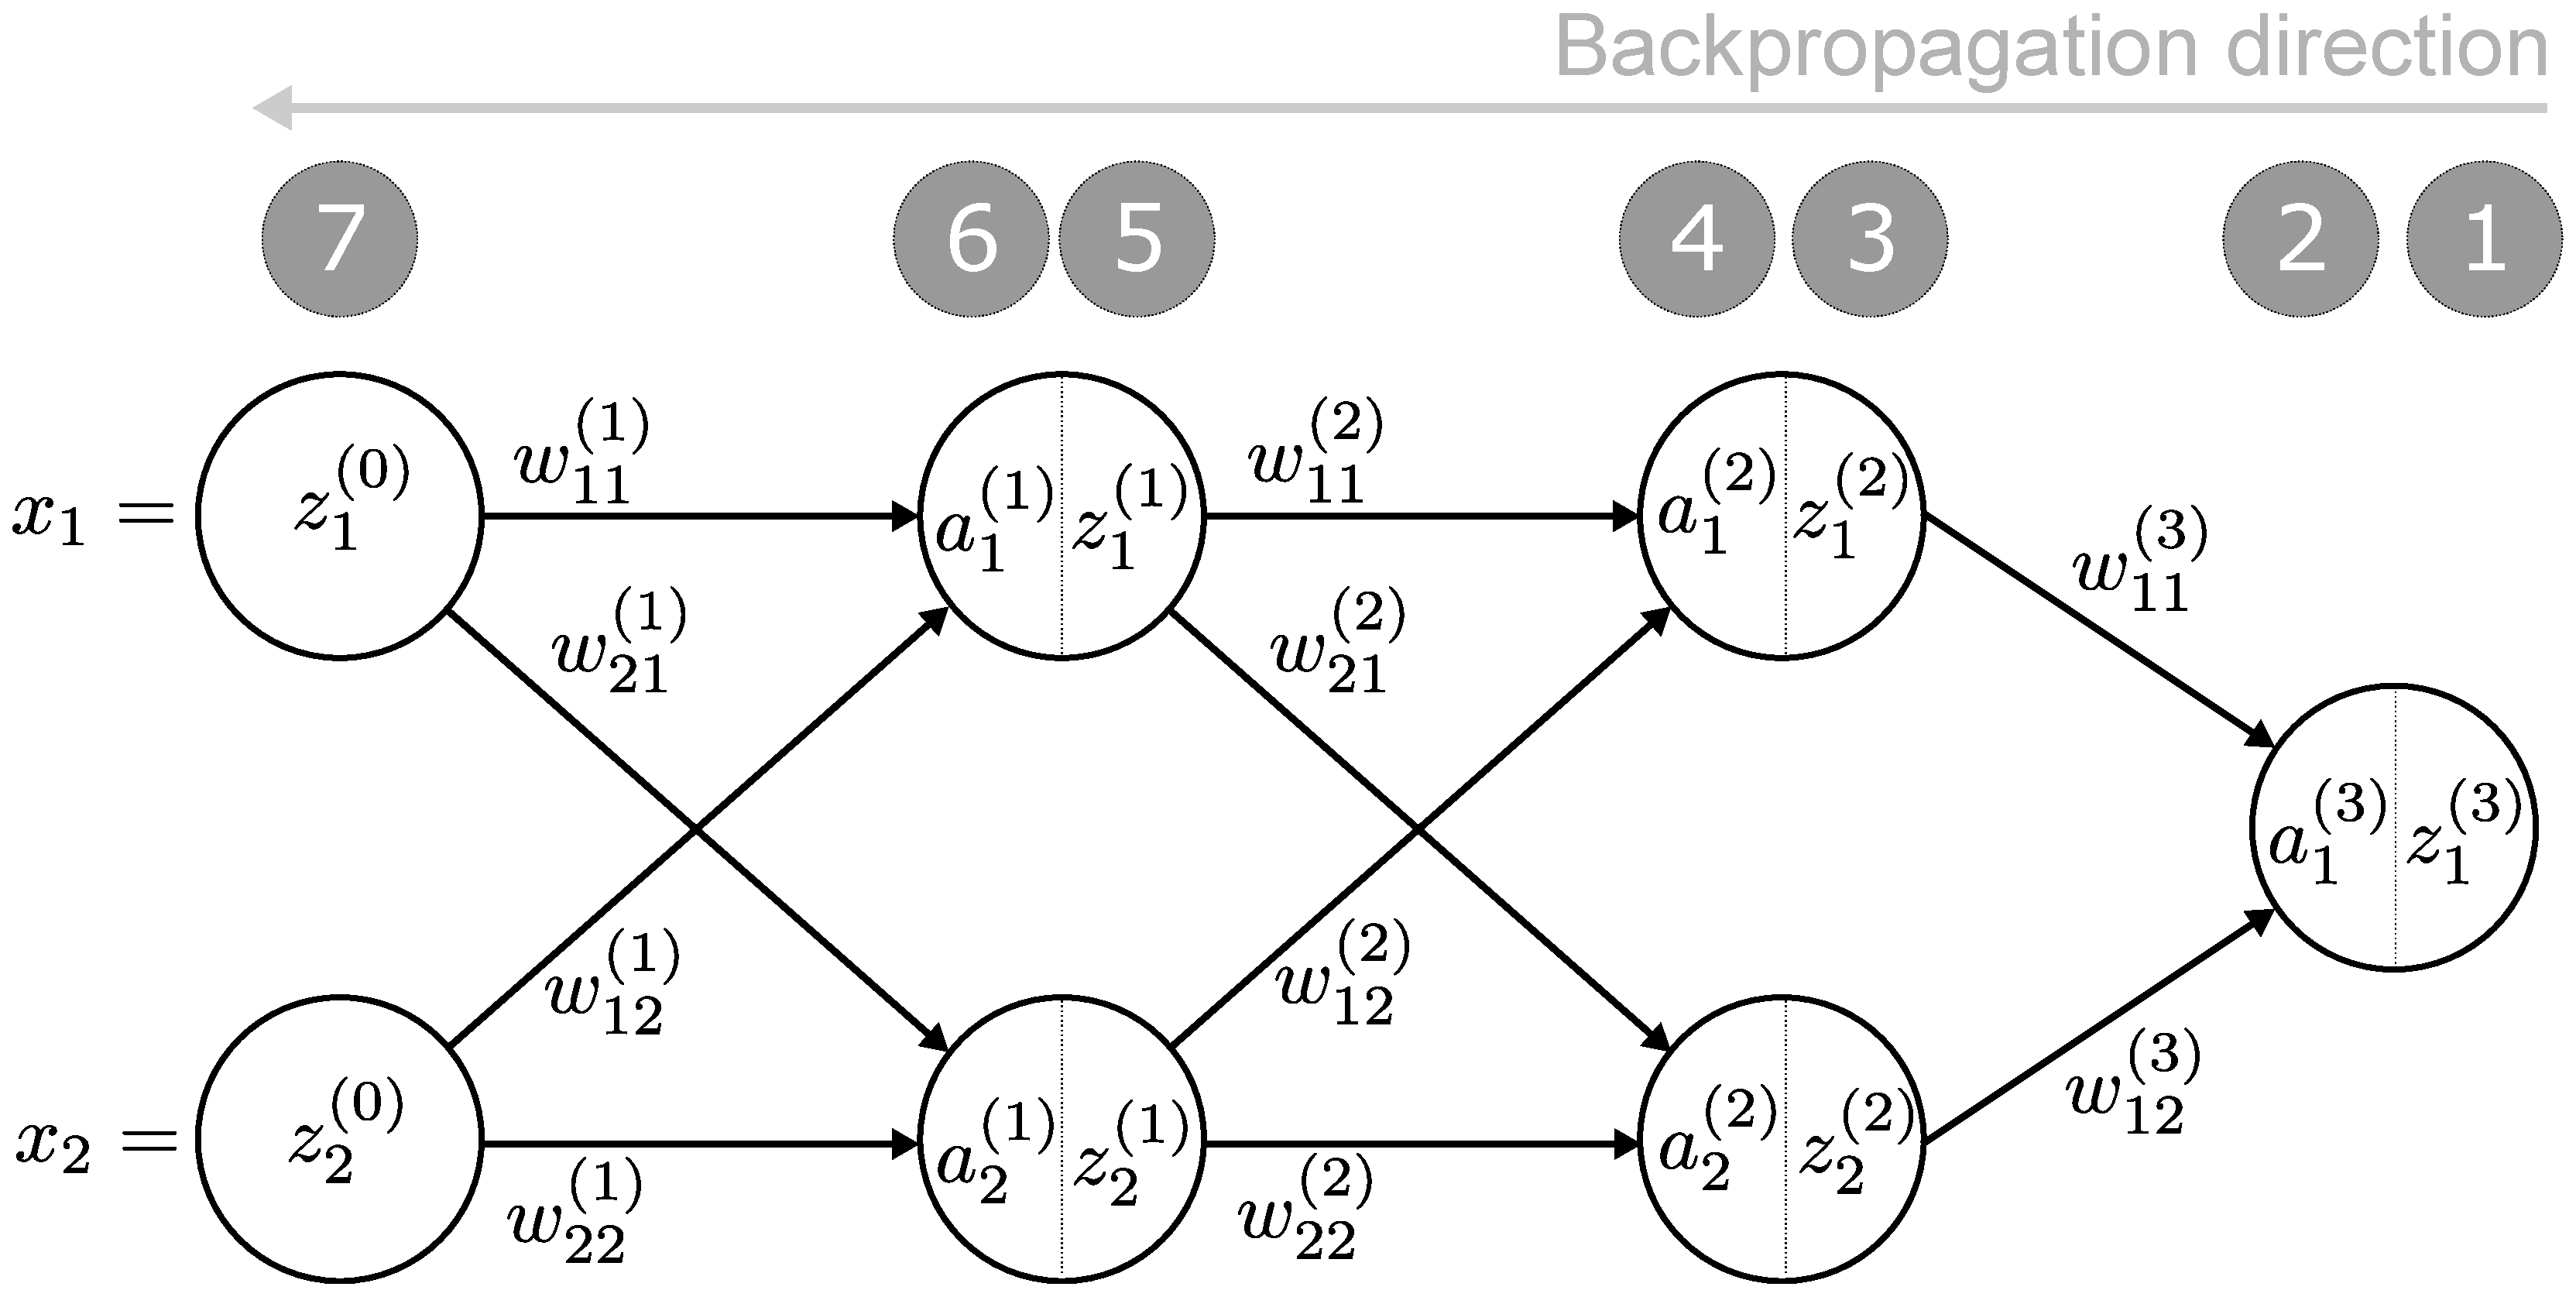
\includegraphics[width=0.9\textwidth]{./neural_networks_labeled_backprop.eps}
\caption{Example neural network}
\label{fig:labeled_backprop}
\end{figure}

We begin by calculating the error, which we assume to be mean square error in this case. We calculate this for a training sample, $(\mathbf{x}, y)$. After the feedforward process is complete, this produces our prediction $\hat{y} = z^{(3)}$. The error is then defined as $E_n = \frac{1}{2}(z^{(3)} - y)^2$. We'll start calculating the derivative of $E_n$ with respect to every value along the way backwards through the neural network. The gradient of $E_n$ with respect to $x^{(3)}$ is simply $\dfrac{\partial E_n}{\partial z^{(3)}} = z^{(3)} - y$. This summarizes all the pieces in Figure \ref{fig:labeled_backprop} for location $1$ in the network.

In step 2, we see that the activation, $a_3$ is the variable of interest. The variable of interest in the last step, $z^{(3)}$ is related to $a^{(3)}$ via the activation function, $z^{(3)} = \sigma(a^{(3)}$. From here we can easily compute $\dfrac{\partial z^{(3)}}{\partial a^{(3)}} = \sigma^{'}(a^{(3)}$, where $\sigma^{'}(\cdot)$ is the derivative of $\sigma(\cdot)$. Now since we know both $\dfrac{\partial E_n}{\partial z^{(3)}}$ from step 1 and $\dfrac{\partial z^{(3)}}{\partial a^{(3)}}$ from this step, we can use the chain rule to write out $\dfrac{\partial E_n}{\partial a^{(3)}} = \dfrac{\partial E_n}{\partial z^{(3)}} \dfrac{\partial z^{(3)}}{\partial a^{(3)}}$. This derivative equals $(z^{(3)} - y) \sigma^{'}(a^{(3)})$ and we see here another reason why we needed to perform forward propagation first - we also need the value of $a^{(3)}$ to compute this derivative.

The value of $\dfrac{\partial E_n}{\partial a^{(3)}}$ is a very important quantity which allows us to calculate the derivatives with respect to the weights of the current layer, for this reason, we give it the shorthand delta notation: $\delta^{(3)} \triangleq \dfrac{\partial E_n}{\partial a^{(3)}}$. Think about the relationship between $a^{(3)}$ and the weights: we know that $a^{(3)} = w_1^{(3)} z_1^{(2)} + w_2^{(3)} z_2^{(2)}$. This means that $\frac{\partial a^{(3)}}{\partial w_1^{(3)}} = z_1^{(2)}$ and$\frac{\partial a^{(3)}}{\partial w_2^{(3)}} = z_2^{(2)}$. More generally, for any layer we can write:

\begin{equation}
    \dfrac{\partial a_i^{(k)}}{\partial w_{ij}^{(k-1)}} = z_j^{(k-1)}
    \label{eq:dadw}
\end{equation}

If we think about our chain rule, once we have $\dfrac{\partial E_n}{\partial a^{(3)}}$ and $\dfrac{\partial a^{(3)}}{\partial w_i^{(3)}}$, then we can calculate $\dfrac{\partial E_n}{\partial w_i^{(3)}}$ with the chain rule by multiplying them together.

We can continue this process stepping backward through the layers through Steps 3 through 7 as well. Let's discuss Step 5, though, because this is where the sum rule comes into play. Once we get to the variable $z_i^{(1)}$ in Figure \ref{fig:labeled_backprop}, we can see that there is not only one pathway back to it, but two pathways back to it: one from node $z_1^{(2)}$ and one from $z_2^{(2)}$. As we discussed earlier, we can apply the chain rule along a single path, but we sum the derivatives across parallel paths back into the same variable. In this case. This is why to calculate this gradient, we sum over all the paths leading back to $z_i^{(1)}$; that is $\dfrac{\partial E_n}{\partial z_i^{(1)}} = \sum\limits_{j=1}^{N_2}\dfrac{\partial E_n}{\partial a_j^{(2)}} \dfrac{\partial a_j^{(2)}}{\partial z_i^{(1)}}$. This can be greatly simplified using the delta notation described earlier and simply becomes $\sum\limits_{j=1}^{N_2} \delta_j^{(2)} w_{ji}^{(2)}$.

\begin{table}[h]
\centering
\caption{Backpropagation Step-by-step, corresponding to each stage in Figure \ref{fig:labeled_backprop}. Step corresponds to the location in the backpropagation process from Figure \ref{fig:labeled_backprop}; Var is the variable that the gradient will be computer with respect to; the local relationship is the relationship of the variable that was the focus of the previous step to that of the current step, which will be connected via the chain rule; the local derivative is the derivative of that local relationship with respect to the variable of interest in this step; and the backpropagated derivative is the the derivative of $E_n$ with respect to the variable of interest in the current step.}
\label{tab:backprop}
\begin{tabular}{llllll}
\toprule
\emph{Step} & \emph{Var} & \emph{Local Relationship} & \emph{Local Derivative} & \emph{Backpropagated Derivative} & \\
\midrule
1 & $z^{(3)}$ & $E_n = \frac{1}{2}(z^{(3)} - y)^2$ & 
$\dfrac{\partial E_n}{\partial z^{(3)}} = z^{(3)} - y$ & 
$\dfrac{\partial E_n}{\partial z^{(3)}} = $ & 
$z^{(3)} - y$ \\[4ex]

2 & $a^{(3)}$ & 
$z^{(3)}=\sigma(a^{(3)})$ & 
$\dfrac{\partial z^{(3)}}{\partial a^{(3)}} = \sigma^{'}(a^{(3)})$ & 
$\dfrac{\partial E_n}{\partial a^{(3)}} = \dfrac{\partial E_n}{\partial z^{(3)}} \dfrac{\partial z^{(3)}}{\partial a^{(3)}}=$ & 
$(z^{(3)} - y) \sigma^{'}(a^{(3)}) \triangleq \delta^{(3)}$ \\[4ex]

3 & $z_i^{(2)}$ & $a^{(3)} = \sum\limits_{j=1}^{N_2} w_j^{(3)} z_j^{(2)}$ & $\dfrac{\partial a^{(3)}}{\partial z_i^{(2)}}= w_i^{(3)}$ & $\dfrac{\partial E_n}{\partial z_i^{(2)}} = \dfrac{\partial E_n}{\partial a^{(3)}} \dfrac{\partial a^{(3)}}{\partial z_i^{(2)}}=$ & 
$ \delta^{(3)} w_i^{(3)}$ \\[4ex]

4 & $a_i^{(2)}$ & 
$z_i^{(2)} = \sigma(a_i^{(2)})$ & 
$\dfrac{\partial z_i^{(2)}}{\partial a_i^{(2)}}= \sigma^{'}(a_i^{(2)})$ & 
$\dfrac{\partial E_n}{\partial a_i^{(2)}} = \dfrac{\partial E_n}{\partial z_i^{(2)}} \dfrac{\partial z_i^{(2)}}{\partial a_i^{(2)}} =$ & 
$\delta^{(3)} w_i^{(3)} \sigma^{'}(a_i^{(2)}) \triangleq \delta_i^{(2)}$ \\[4ex]

5 & $z_i^{(1)}$ &
$a_j^{(2)} = \sum\limits_{k=1}^{N_1} w_{jk}^{(2)} z_k^{(1)}$ & 
$\dfrac{\partial a_j^{(2)}}{\partial z_i^{(1)}} = w_{ji}^{(2)}$ & 
$\dfrac{\partial E_n}{\partial z_i^{(1)}} = \sum\limits_{j=1}^{N_2}\dfrac{\partial E_n}{\partial a_j^{(2)}} \dfrac{\partial a_j^{(2)}}{\partial z_i^{(1)}} =$ & 
$\sum\limits_{j=1}^{N_2} \delta_j^{(2)} w_{ji}^{(2)}$\\[4ex]

6 & $a_i^{(1)}$ & 
$z_i^{(1)} = \sigma(a_i^{(1)})$ &
$\dfrac{\partial z_i^{(1)}}{\partial a_i^{(1)}} = \sigma^{'}(a_i^{(1)})$ &
$\dfrac{\partial E_n}{\partial a_i^{(1)}} = \dfrac{\partial E_n}{\partial z_i^{(1)}} \dfrac{\partial z_i^{(1)}}{\partial a_i^{(1)}}= $& 
$\sigma^{'}(a_i^{(1)}) \sum\limits_{j=1}^{N_2} \delta_j^{(2)} w_{ji}^{(2)} \triangleq \delta_i^{(1)}$ \\[4ex]

7 & $x_i$ &
$a_j^{(1)} = \sum\limits_{k=1}^{N_0} w_{jk}^{(1)} x_k$ & 
$\dfrac{\partial a_j^{(1)}}{\partial z_i^{(0)}} = w_{ji}^{(1)}$ & 
$\dfrac{\partial E_n}{\partial x_i} = \sum\limits_{j=1}^{N_1}\dfrac{\partial E_n}{\partial a_j^{(1)}} \dfrac{\partial a_j^{(1)}}{\partial x_i} =$ & 
$\sum\limits_{j=1}^{N_1} \delta_j^{(1)} w_{ji}^{(1)}$ \\[4ex]

\bottomrule
\end{tabular}
\end{table}

All of the expressions found in Table \ref{tab:backprop} are also presented in Table \ref{tab:matrix} in matrix form  (where applicable in Steps 3-7 since 1 and 2 are scalar only) and provide a more convenient means of implementing these equations. In this table, not that the symbol $\circ$ represents the Hadamard Product, which is simply the element-wise product of two matrices. As an example:

\begin{equation}
    \begin{bmatrix}
        x_1 \\
        x_2 \\
        x_3
    \end{bmatrix} \circ
    \begin{bmatrix}
        y_1 \\
        y_2 \\
        y_3
    \end{bmatrix} = 
    \begin{bmatrix}
        x_1y_1 \\
        x_2y_2 \\
        x_3y_3
    \end{bmatrix}
\end{equation}



% This table is for the matrix forms of the backpropagation equations
\begin{table}[h]
\centering
\label{tab:matrix}
\caption{\emph{Backpropagation Equations in Matrix Form.} For each of the steps in Figure \ref{fig:labeled_backprop}, this table provides the matrix form of the equations for convenient implementation.}
\begin{tabular}{lll}
\toprule
\emph{ID} & \emph{Derivative} & \emph{Matrix Forms} \\
\midrule
1 & $\dfrac{\partial E_n}{\partial z^{(3)}} =$ & $z^{(3)} - y$ \\[4ex]

2 & $\dfrac{\partial E_n}{\partial a^{(3)}} = \dfrac{\partial E_n}{\partial z^{(3)}} \dfrac{\partial z^{(3)}}{\partial a^{(3)}}=$ & $(z^{(3)} - y) \sigma^{'}(a^{(3)}) \triangleq \delta^{(3)}$  \\[4ex]

3 & $\dfrac{\partial E_n}{\partial \mathbf{z}^{(2)}} = \dfrac{\partial E_n}{\partial a^{(3)}} \dfrac{\partial a^{(3)}}{\partial \mathbf{z}^{(2)}} =$ & $ \delta^{(3)} \mathbf{w}^{(3)}$  \\[4ex]

4 & $\dfrac{\partial E_n}{\partial \mathbf{a}^{(2)}} = \dfrac{\partial E_n}{\partial \mathbf{z}^{(2)}} \dfrac{\partial \mathbf{z}^{(2)}}{\partial \mathbf{a}^{(2)}} =$ & $ \delta^{(3)} \mathbf{w}^{(3)} \circ \sigma^{'}(\mathbf{a}^{(2)}) \triangleq \bm{\delta}^{(2)}$  \\[4ex]

5 & $\dfrac{\partial E_n}{\partial \mathbf{z}^{(1)}} = \dfrac{\partial E_n}{\partial \mathbf{a}^{(2)}} \dfrac{\partial \mathbf{a}^{(2)}}{\partial \mathbf{z}^{(1)}}=$ & $ {\mathbf{W}^{(2)}}^{\top} \bm{\delta}^{(2)}$  \\[4ex]

6 &  $\dfrac{\partial E_n}{\partial \mathbf{a}^{(1)}} = \dfrac{\partial E_n}{\partial \mathbf{z}^{(1)}} \dfrac{\partial \mathbf{z}^{(1)}}{\partial \mathbf{a}^{(1)}} =$ & $ {\mathbf{W}^{(2)}}^{\top} \bm{\delta}^{(2)} \circ \sigma^{'}(\mathbf{a}^{(1)}) \triangleq \bm{\delta}^{(1)}$ \\[4ex]

7 & $\dfrac{\partial E_n}{\partial \mathbf{x}} =\dfrac{\partial E_n}{\partial \mathbf{a}^{(1)}} \dfrac{\partial \mathbf{a}^{(1)}}{\partial \mathbf{x}}=$ & $ {\mathbf{W}^{(1)}}^{\top} \bm{\delta}^{(1)}$ \\[4ex]

\bottomrule
\end{tabular}
\end{table}

\section{Summary of the general equations for forward and backpropagation}

So far, we've focused on the example shown in \ref{fig:labeled_backprop}, however, most of the equations we described here are far more generally applicable. Here we go through the general equations for forward and backpropagation

\subsection{General forward propagation}

For forward propagation, considering the Figure \ref{fig:ff}, starting with our input $\mathbf{z}^{(0)} = \mathbf{x}$, we can compute all of the values of the following layers using the following two equations and alternating between them. First, calculate the activations for the next layer:

\begin{equation}
    a_i^{(k)} = \sum_{j=1}^{N_{k-1}} w_{ij}^{(k)} z_j^{(k-1)} 
\end{equation}

Or in matrix form:

\begin{equation}
    \mathbf{a}^{(k)} = \mathbf{W}^{(k)} \mathbf{z}^{(k-1)}
\end{equation}

Then calculate the activated node value in that next layer:

\begin{equation}
    z_i^{(k)} = \sigma(a_i^{(k)})
\end{equation}

\begin{equation}
    \mathbf{z}^{(k)} = \sigma(\mathbf{a}^{(k)})
\end{equation}

\subsection{General backpropagation}

Let's focus on the right-hand side of the node highlighted in Figure \ref{fig:focused}. We focus on that in Figure \ref{fig:backprop}, looking at how the node $z_i^{(k)}$ is connected to each of the nodes in proceeding layer ($k+1$). 

\begin{figure}[h]
\centering
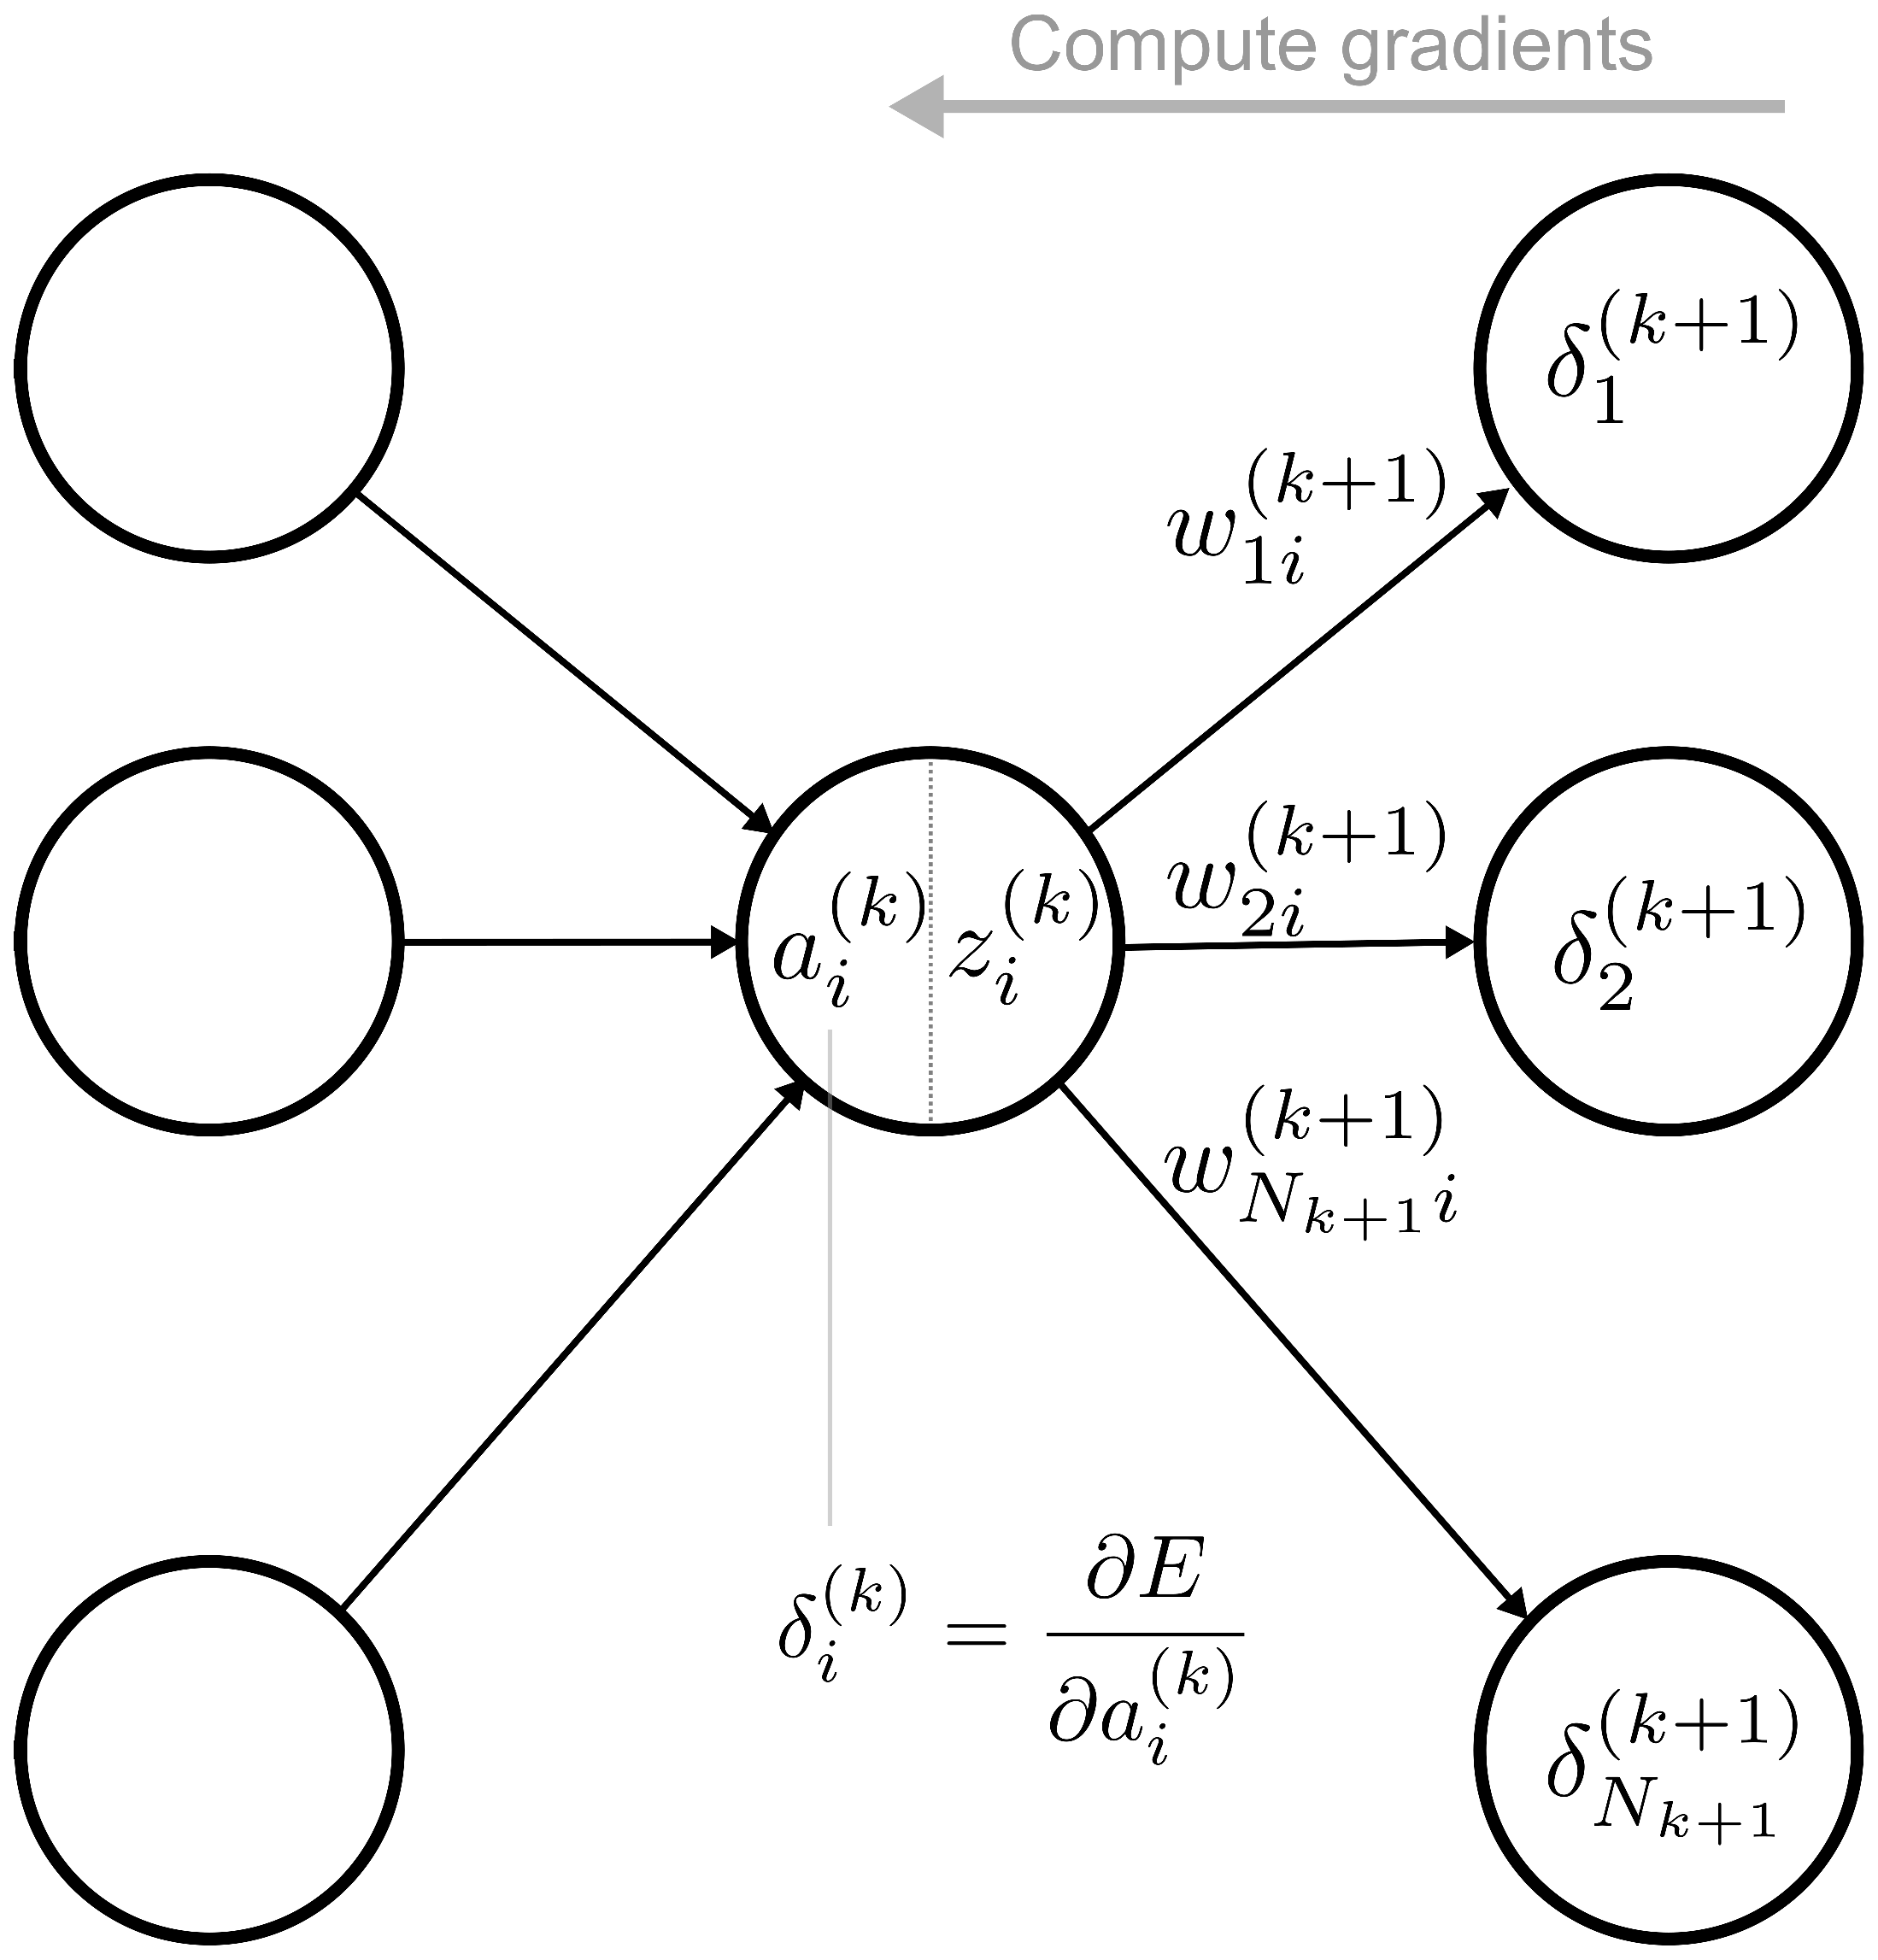
\includegraphics[width=0.45\textwidth]{./neural_networks_local_backpropagation.eps}
\caption{Example neural network}
\label{fig:backprop}
\end{figure}

Given Eq. \ref{eq:dadw} and the definition of $\delta_i^{(k)}$:

\begin{equation}
    \delta_i^{(k)} = \dfrac{\partial E}{\partial a_i^{(k)}} = \sigma^{'}(a_i^{(k)}) \sum\limits_{j=1}^{N_k} \delta_j^{(k+1)}w_{ji}^{(k+1)}
\end{equation}

Or in matrix form:

\begin{equation}
     \bm{\delta}^{(k)} \triangleq \dfrac{\partial E}{\partial \mathbf{a}^{(k)}} = {\mathbf{W}^{(k+1)}}^{\top} \bm{\delta}^{(k+1)} \circ \sigma^{'}(\mathbf{a}^{(k)}) 
\end{equation}

We can use these to calculate the derivative with respect to any weight:

\begin{equation}
    \dfrac{\partial E_n}{\partial w_{ij}^{(k)}} = 
    \dfrac{\partial E_n}{\partial a_i^{(k)}} \dfrac{\partial a_i^{(k)}}{\partial w_{ij}^{(k)}} = \delta_i^{(k)} z_j^{(k-1)}
\end{equation}

Or in matrix form where the $(i,j)^{\mathrm{th}}$ element of this matrix is $\frac{\partial E_n}{\partial w_{ij}}$:

\begin{equation}
    \dfrac{\partial E_n}{\partial \mathbf{w}^{(k)}} = \bm{\delta}^{(k)} {\mathbf{z}^{(k-1)}}^{\top}
\end{equation}

The process of backpropagation is sequentially applying these equations moving backwards through the neural network, then once all of the derivatives with respect to the activations have been calculated, calculate the derivatives with respect to each of the weights. These values can then be used in the gradient descent process to update the weights themselves and fit the neural network to the training data.

\nocite{*}

\bibliography{references}{}
\bibliographystyle{plain}

\clearpage
\section{Summary and quick reference}
\begin{table}[htb!]
\begin{tabular}{ll}
\parbox[b][0.4\textheight][t]{0.47\textwidth}{
\subsection{Forward Propagation}
    Forward propagation is the iterative application of the following two equations:
        \begin{align*}
            a_i^{(k)} &= \sum_{j=1}^{N_{k-1}} w_{ij}^{(k)} z_j^{(k-1)} \\
            z_i^{(k)} &= \sigma(a_i^{(k)})
        \end{align*}
        
        In matrix form those equations are:
        
        \begin{align*}
            \mathbf{a}^{(k)} &= \mathbf{W}^{(k)} \mathbf{z}^{(k-1)} \\
            \mathbf{z}^{(k)} &= \sigma(\mathbf{a}^{(k)})
        \end{align*}
} &
\parbox[b][0.4\textheight][t]{0.47\textwidth}{
        \centering
        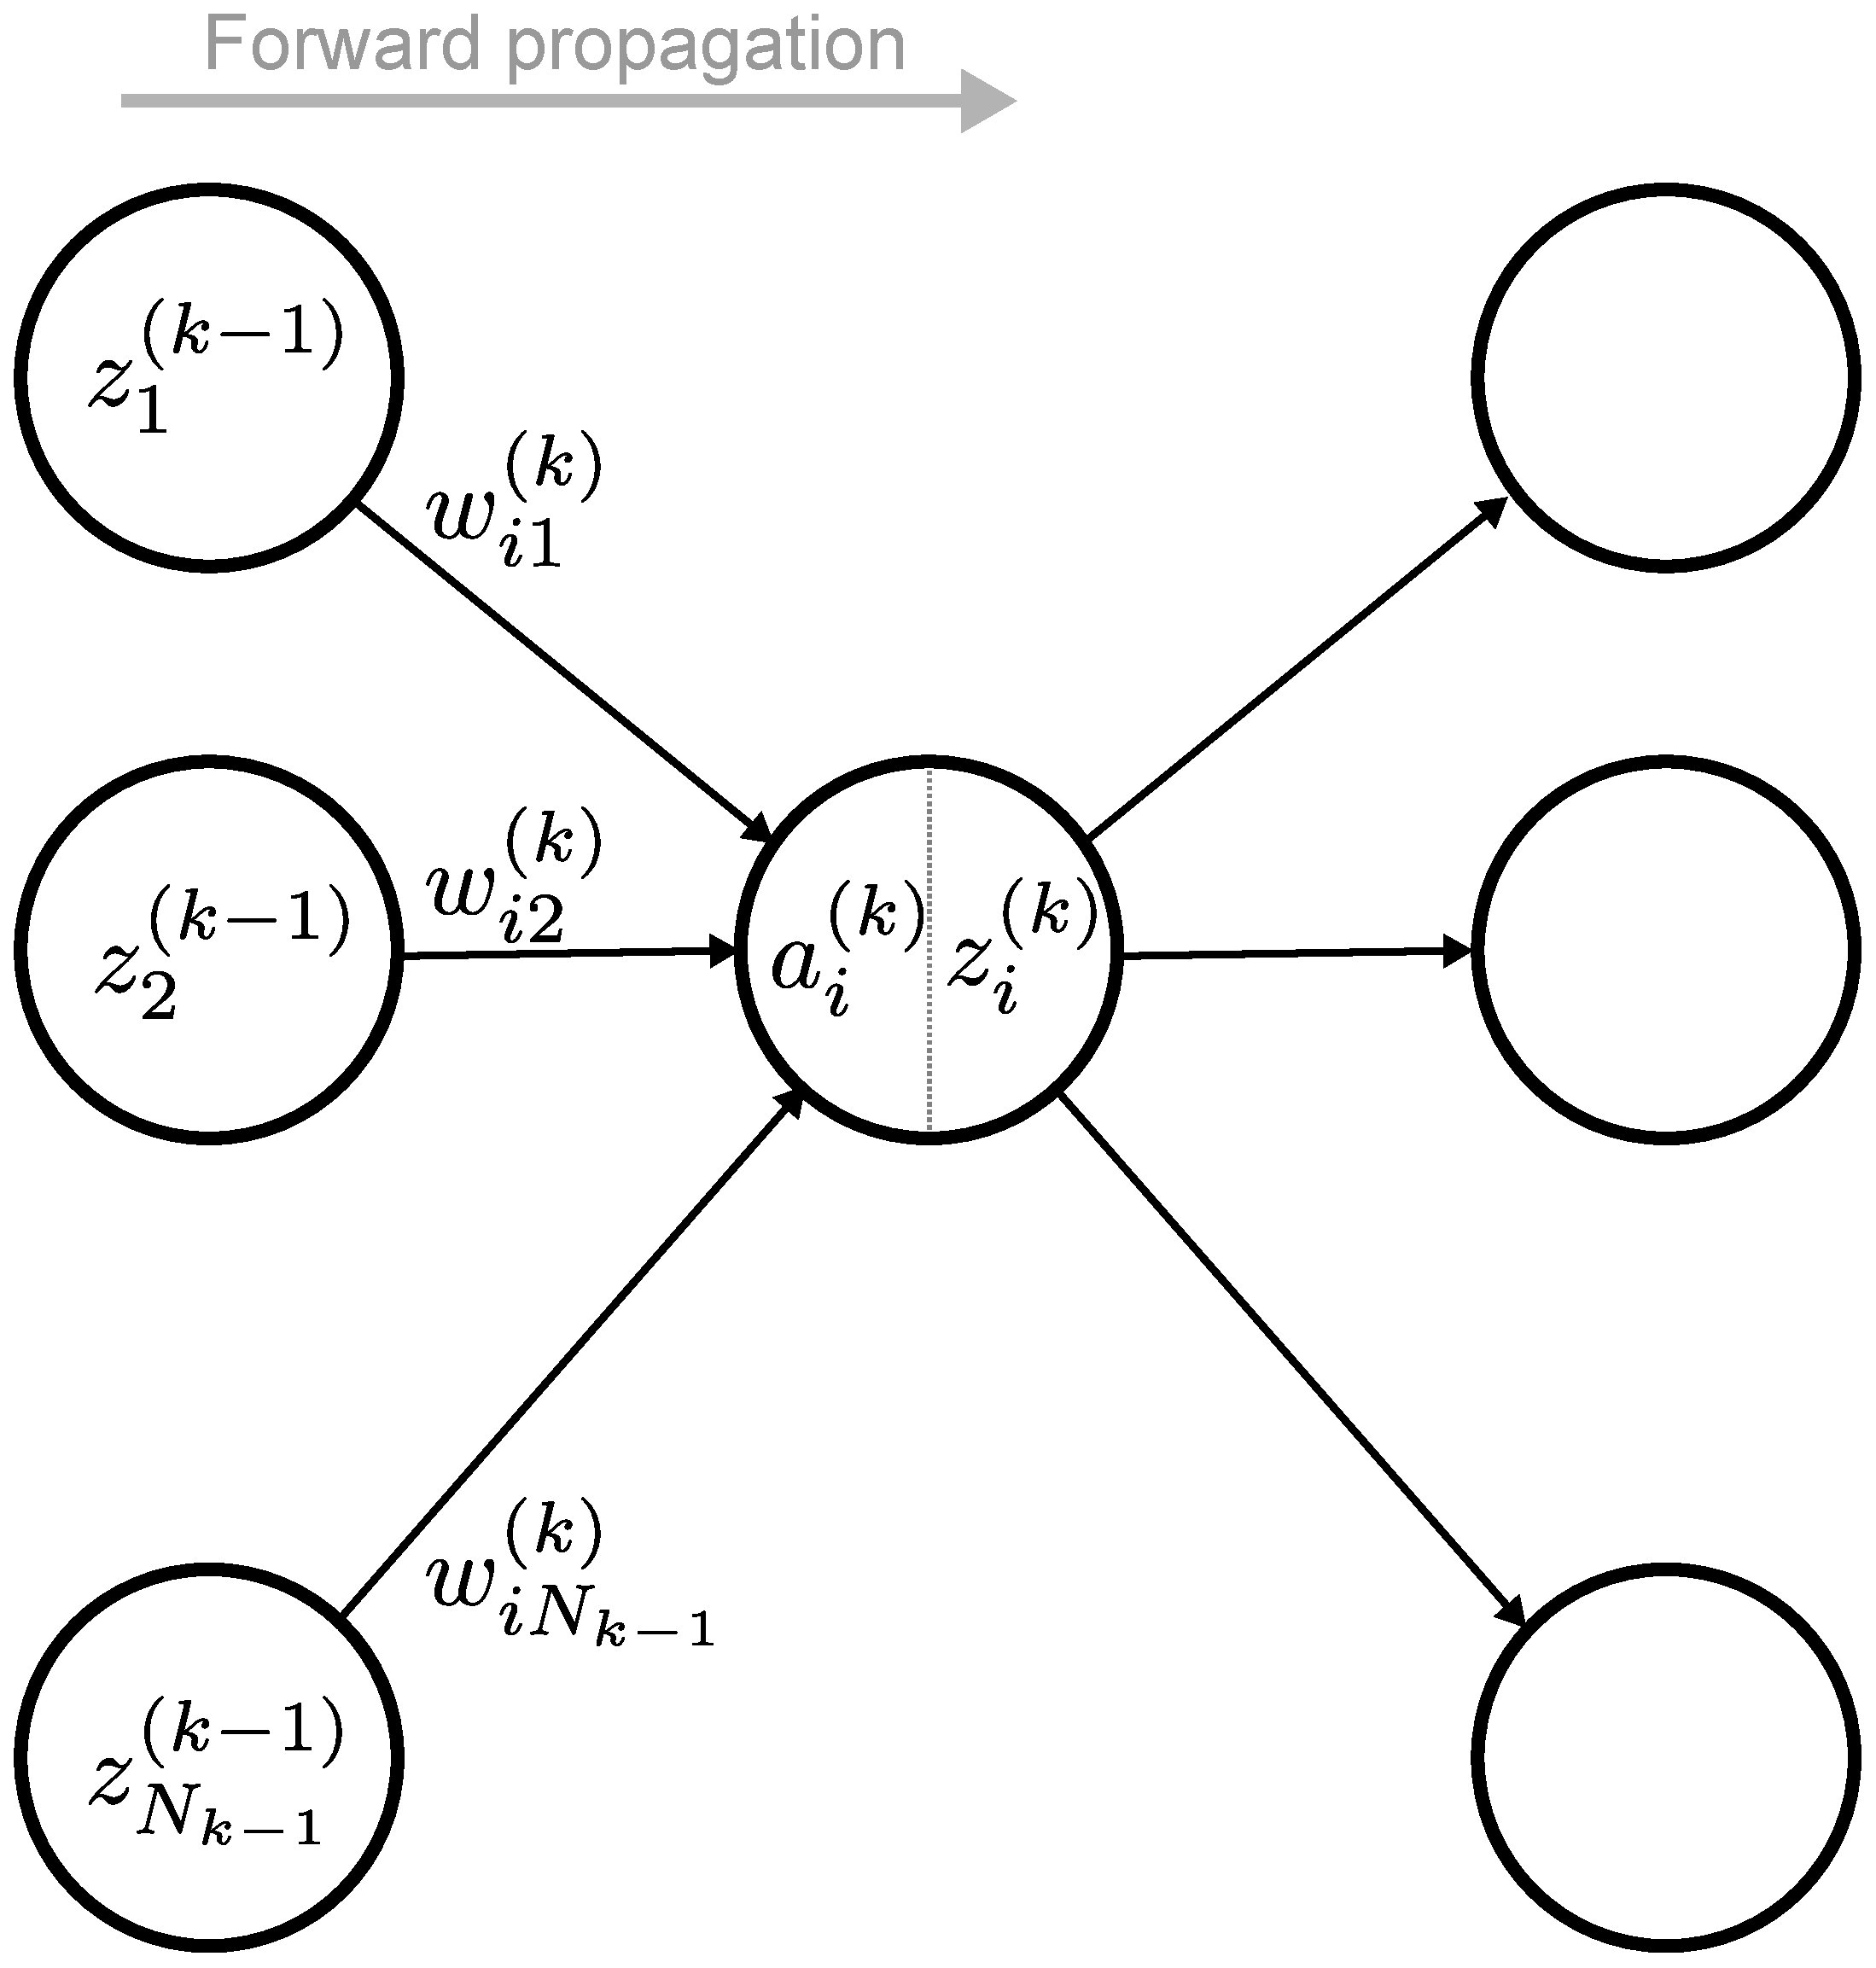
\includegraphics[width=\linewidth]{./neural_networks_local_forward_propagation.eps}
        \caption{Forward propagation}
        \label{fig:fp}
}
\\
\parbox[b][0.4\textheight][t]{0.47\textwidth}{
    \subsection{Backpropagation}
    Backpropagation begins with the calculation of the gradient of the error with respect to the final set of activations, which for mean square error with sigmoidal activation and $K$-layer neural network is:
    \begin{equation*}
        \delta_i^{(K)} \triangleq \dfrac{\partial E_n}{\partial a_i^{(K)}} = (z_i^{(3)} - y_i) \sigma^{'}(a_i^{(3)})
    \end{equation*}
    We then propagate that back through the neural network and calculate the gradients with respect to each weight along the way (for $k = K-1,...1$):
    
    \begin{align*}
        \delta_i^{(k)} \triangleq \dfrac{\partial E_n}{\partial a_i^{(k)}} &= \sigma^{'}(a_i^{(k)}) \sum\limits_{j=1}^{N_{k+1}} \delta_j^{(k+1)} w_{ji}^{(k+1)} \\
        \dfrac{\partial E_n}{\partial w_{ij}^{(k)}} &= 
        \dfrac{\partial E_n}{\partial a_i^{(k)}} \dfrac{\partial a_i^{(k)}}{\partial w_{ij}^{(k)}} = \delta_i^{(k)} z_j^{(k-1)}
    \end{align*}
    
    Or in matrix form:
    
    \begin{align*}
         \bm{\delta}^{(k)} \triangleq \dfrac{\partial E_n}{\partial \mathbf{a}^{(k)}} &= {\mathbf{W}^{(k+1)}}^{\top} \bm{\delta}^{(k+1)} \circ \sigma^{'}(\mathbf{a}^{(k)}) \\
         \dfrac{\partial E_n}{\partial \mathbf{w}^{(k)}} &= \bm{\delta}^{(k)} {\mathbf{z}^{(k-1)}}^{\top}
    \end{align*}

} &
\parbox[b][0.4\textheight][t]{0.47\textwidth}{
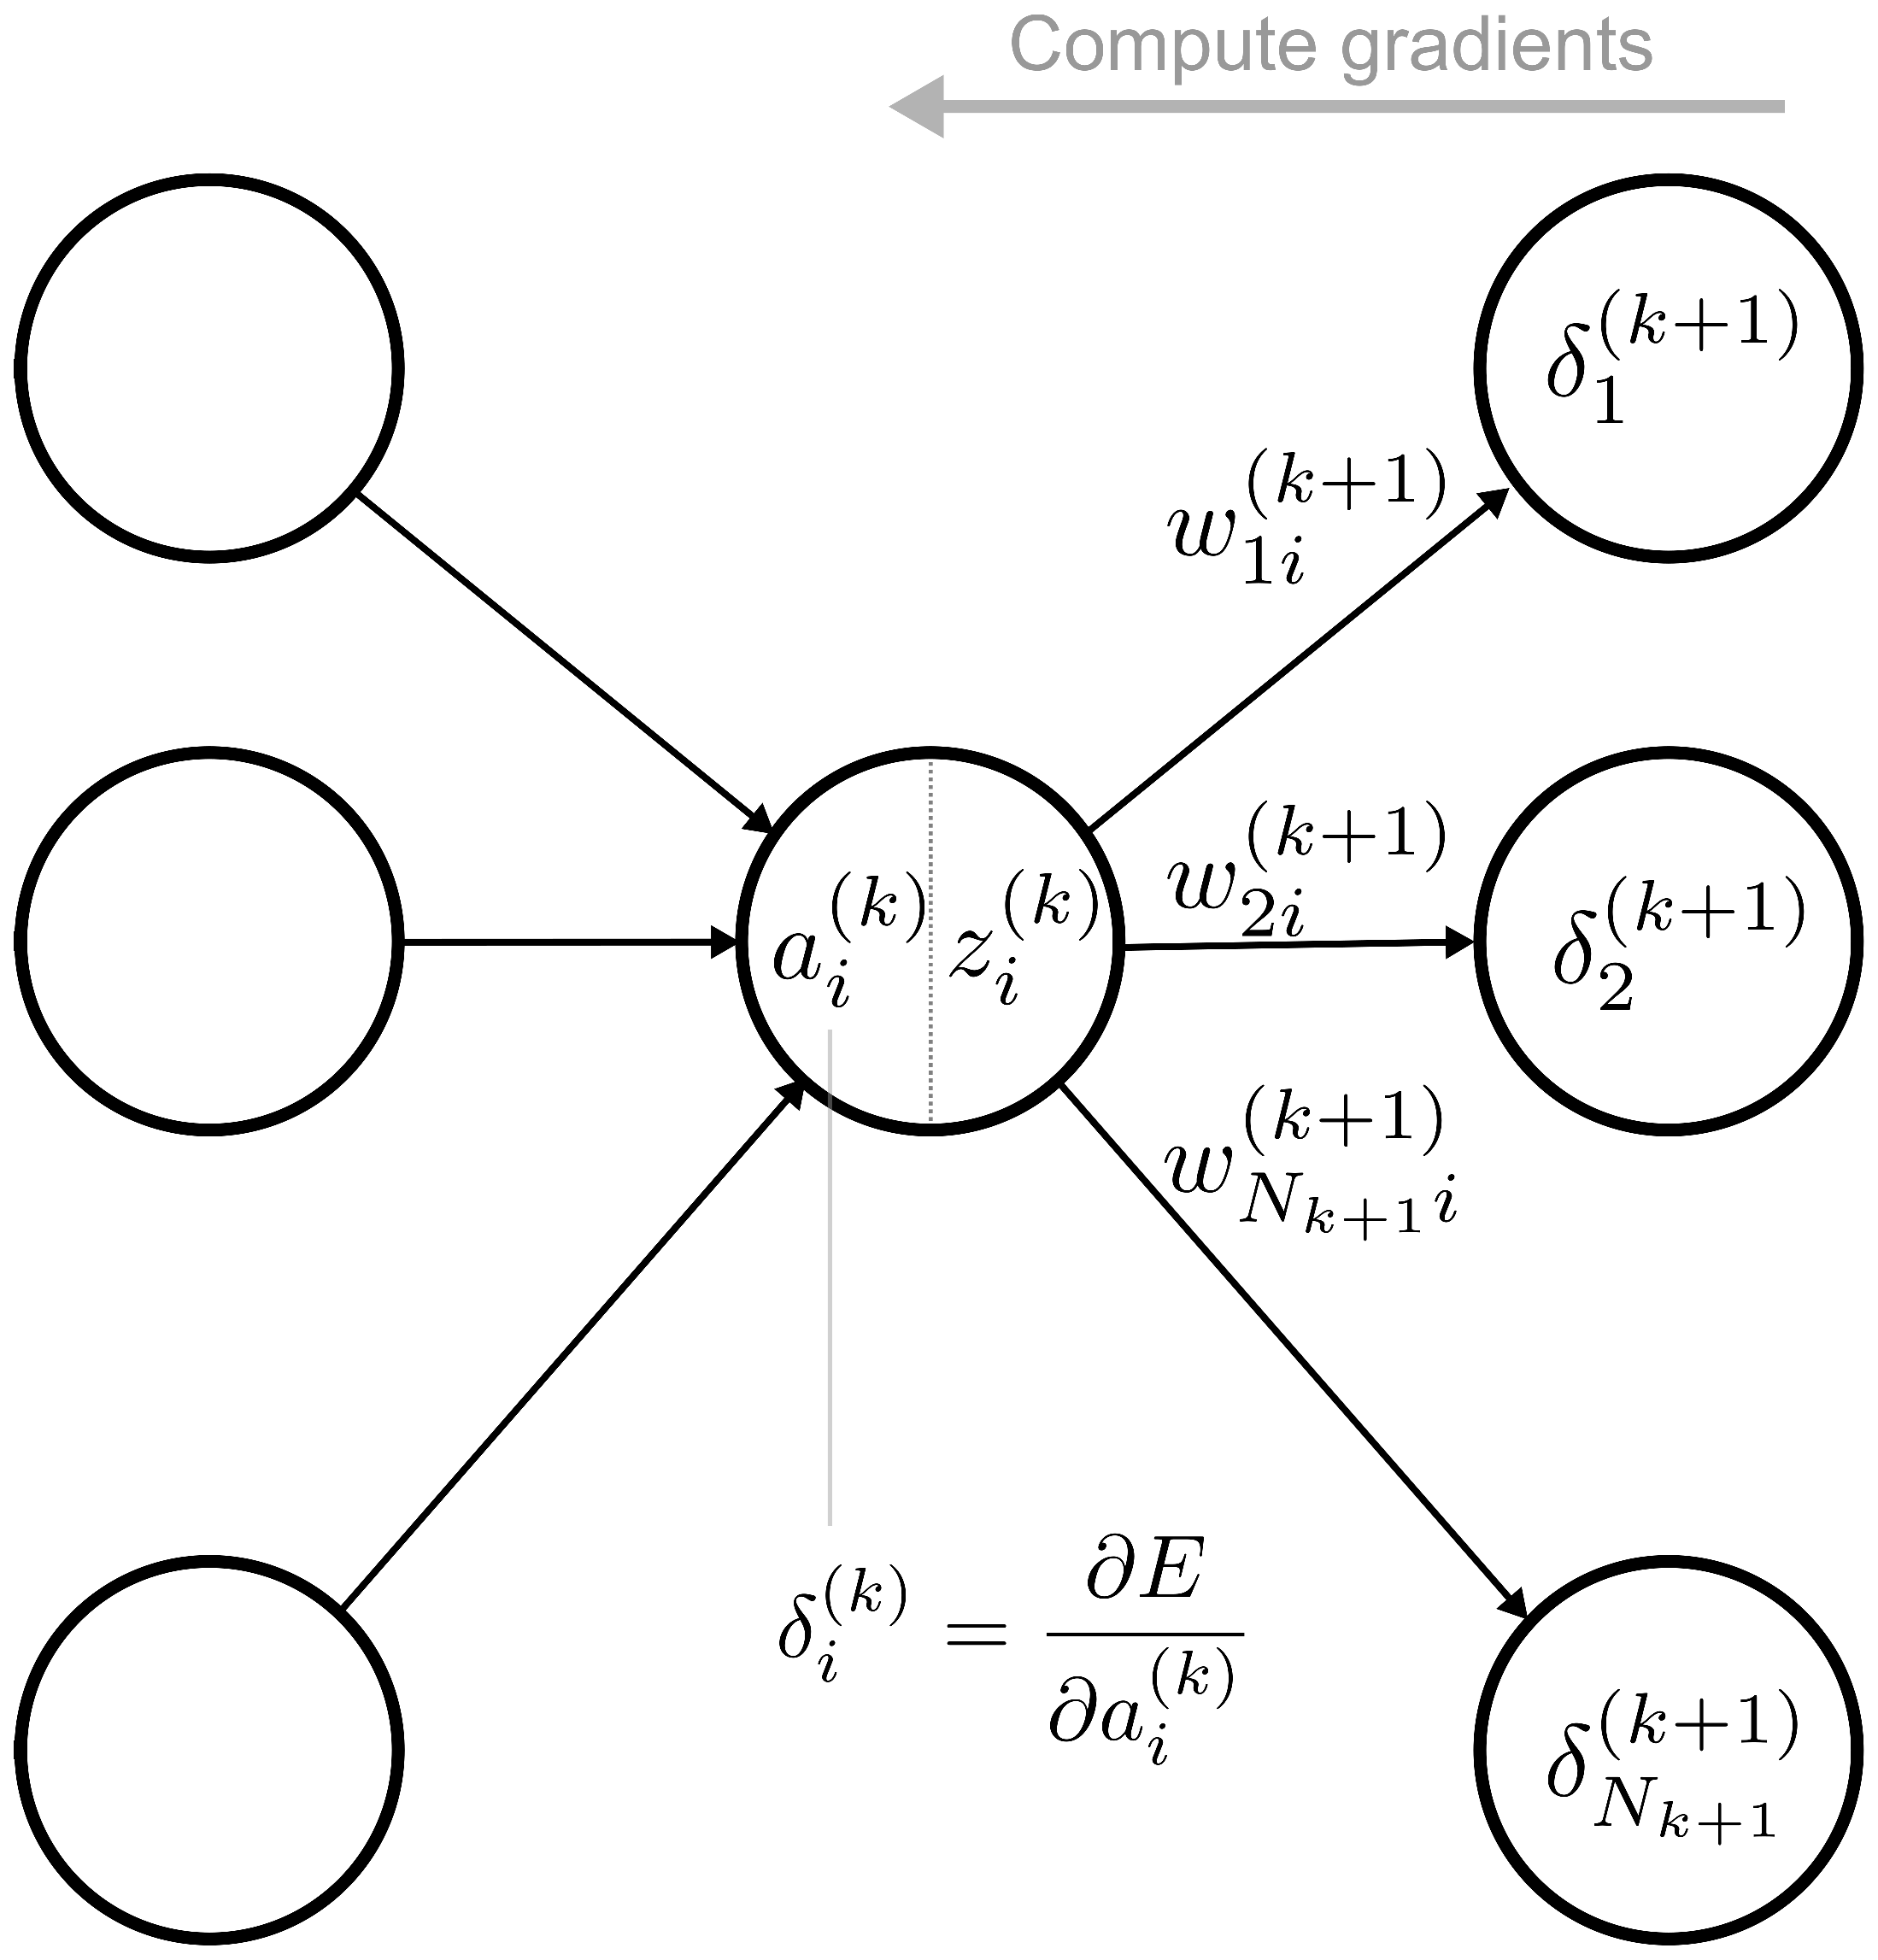
\includegraphics[width=\linewidth]{./neural_networks_local_backpropagation.eps} }
\end{tabular}
\end{table}

\end{document}


